\chapter{Controllo del moto}
\paragraph{}
Il problema del controllo di un manipolatore consiste nel determinare l'andamento delle forze generalizzate che gli attuatori devono applicare ai giunti in modo da garantire, con il soddisfacimento di specifiche assegnate sul transitorio e sul regime, l'esecuzione delle operazioni comandate.

Le operazioni consistono nell'esecuzione di moti assegnati al manipolatore che comprenderanno due aspetti:
\begin{itemize}
	\item moto dell'organo terminale nello \emph{spazio libero}.
	\item moto dell'organo terminale nell'interazione con \emph{l'ambiente}.
\end{itemize} 
Le tecniche di controllo possono essere,
\begin{itemize}
	\item nello \emph{\textbf{spazio dei giunti}}, dove possiamo distinguere:
	\begin{itemize}
		\item Controllo \emph{centralizzato} in cui si tiene conto degli effetti dinamici di interazione con gli altri giunti.
		\item Controllo \emph{decentralizzato} in cui il singolo giunto del manipolatore viene controllato in maniera indipendente dal moto degli altri giunti. 
	\end{itemize}
	\item e direttamente nello \emph{\textbf{spazio operativo}}.
\end{itemize}

\section{Tecniche di controllo del moto}
In generale, \emph{le caratteristiche di moto} sono specificate nello spazio operativo, le \emph{azioni di controllo} vengono esplicate in maniera diretta nello spazio dei giunti mediante le forze generalizzate sviluppate dagli attuatori. Questa caratteristica porta ad individuare due modalità di controllo illustrate di seguito.

\subsubsection{\underline{Controllo nello spazio dei giunti:}} 
Si articola in due sottoproblemi:
\begin{enumerate}
	\item Inversione della cinematica del manipolatore per la traduzione delle specifiche di moto, generate nello spazio operativo $\underline{x}_{\,d}$ (desiderata), in grandezze di riferimento espresse nello spazio dei giunti $\underline{q}_{\,d}$ (desiderata);
	\item Realizzazione di un sistema di controllo nello spazio dei giunti che deve garantire l'inseguimento dei riferimenti da parte delle grandezze controllate $\underline{q}$.
\end{enumerate}

\begin{center}
	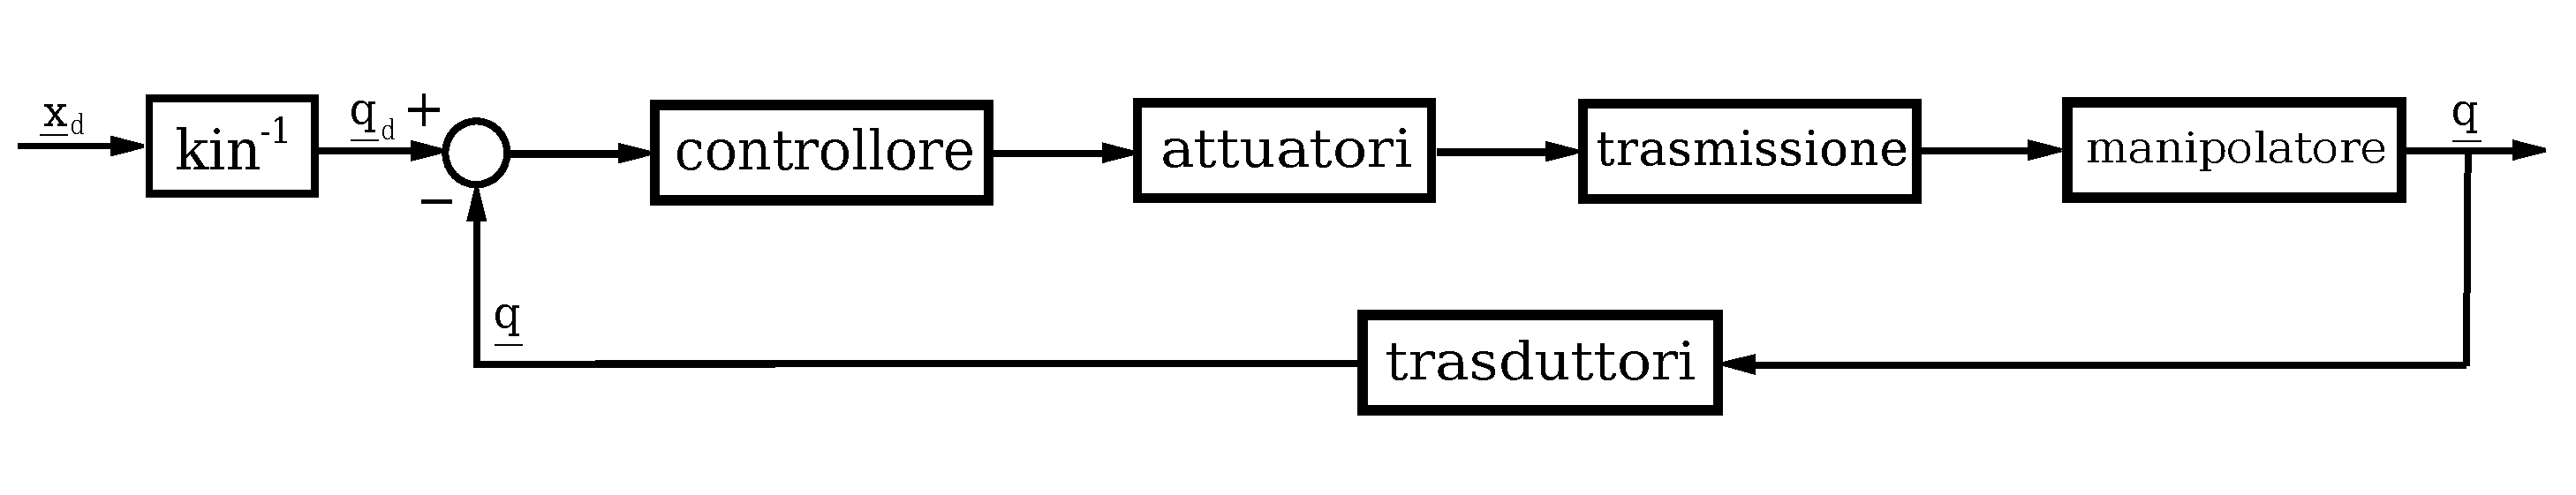
\includegraphics[scale=0.25]{schemaSpazioDeiGiunti.pdf}
	\caption{Schema di principio di controllo nello spazio dei giunti.}
\end{center}

\subsubsection{\underline{Controllo nello spazio operativo:}}
Questa soluzione segue un approccio di tipo globale che richiede una maggiore complessità algoritmica, con tale soluzione infatti, l'inversione cinematica è implicitamente assunta interna all'anello di controllo.

\begin{center}
	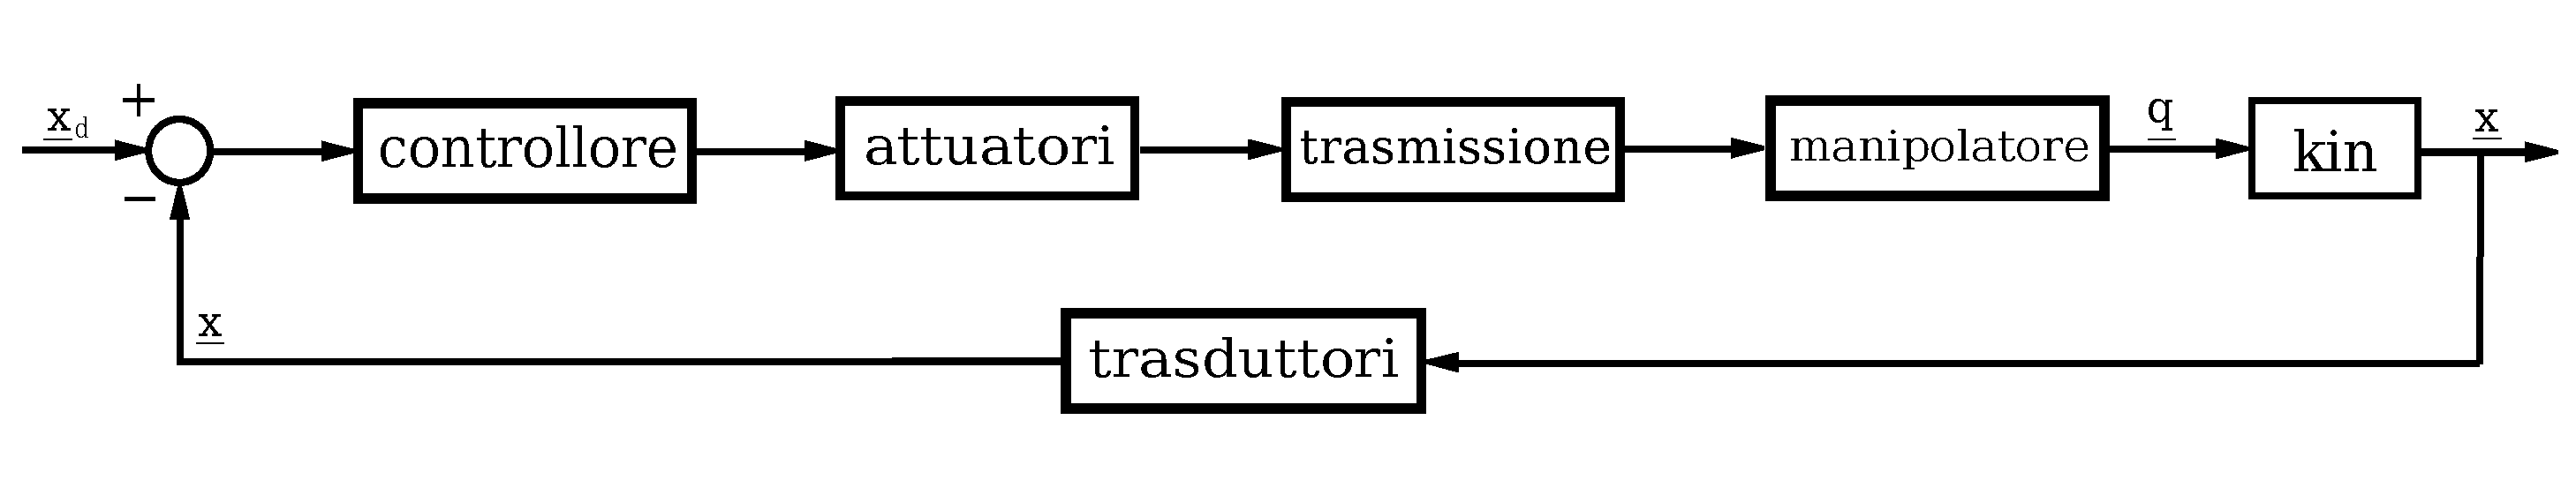
\includegraphics[scale=0.25]{schemaSpazioOperativo.pdf}
	\caption{Schema di principio di controllo nello spazio operativo.}
\end{center}

\subsubsection{\underline{Discorso qualitativo:}}
Le specifiche di moto sono usualmente prescritte nello spazio operativo e come si nota nella Figura 9.1 è pertanto necessario utilizzare un algoritmo di inversione cinematica per poter ricavare i riferimenti degli schemi di controllo operanti nello spazio dei giunti. Questa inversione presenta un carico computazionale notevole, specie se si richiede anche l'inversione della cinematica differenziale del primo e del secondo ordine (velocità e accelerazione). 

Un approccio alternativo consiste nel considerare schemi di controllo sviluppati direttamente nello spazio operativo, come illustrato nella Figura 9.2. L'impiego di tali schemi è vantaggioso quando ci poniamo il problema del controllo del manipolatore in situazioni di \emph{interazione con l'ambiente}. 

Gli schemi di controllo nello spazio operativo sono basati sul confronto diretto degli ingressi, che specificano le traiettorie nello spazio operativo, con le misure delle corrispondenti grandezze di uscita del manipolatore. Ne consegue che nel controllore devono essere presenti delle azioni che consentono di passare dallo spazio operativo, in cui è valutato l'errore di inseguimento, allo spazio dei giunti, in cui sono esplicate le forze generalizzate di controllo.

\section{Controllo Decentralizzato}
Iniziamo trattando il controllo nello spazio dei giunti, in particolare illustriamo la tecnica del controllo decentralizzato. Riscriviamo le equazioni del moto di un manipolatore completo di attuatori (motori) $(8.47)$ trascurando le forze esterne e le forze di attrito statico,
\begin{equation}
	B(\underline{q})\ddot{\underline{q}} + C(\underline{q}, \underline{\dot{q}}) \underline{\dot{q}} + \underline{g}(\underline{q}) + F_v \,\underline{\dot{q}} = \underline{\tau}   
\end{equation}

\paragraph{}
Controllare il moto di un manipolatore nello spazio libero significa determinare le $n$ componenti di forza generalizzata, (\emph{coppie per i giunti rotoidali e forze per i giunti prismatici}), che consentono di realizzare un moto $\underline{q}(t)$ tale che risulti $\underline{q}(t) = \underline{q}_{\,d}(t)$. Con $\underline{q}_{\,d}(t)$ indichiamo il vettore delle  variabili di giunto con le $n$ traiettorie di riferimento specificate per gli $n$ giunti.

\paragraph{}
Sia $\underline{q}_{\,m}$ il vettore delle variabili di posizione dei motori, sia $\underline{q}$ il vettore delle coordinate dei giunti e sia $K_r$ la matrice dei rapporti di trasmissione, otteniamo le seguenti relazioni,
\begin{equation}
	\underline{q}_{\,m} = K_r \underline{q} \qquad \qquad \underline{q} = K_r^{-1} \underline{q}_{\,m}
\end{equation}
sia $\underline{\tau}_{\,m}$ il vettore delle azioni sui motori e sia $\underline{\tau}$ il vettore delle azioni sui giunti, facciamo qualche considerazione energetica eguagliando la potenza erogata nello spazio dei giunti e la potenza erogata nello spazio dei motori,
\begin{equation*}
	P = \underline{\tau}^T \underline{\dot{q}} = \underline{\tau}_{\,m}^T \underline{\dot{q}}_{\,m} \quad \Rightarrow \quad \underline{\tau}^T \underline{\dot{q}} = \underline{\tau}_{\,m}^T K_r \underline{\dot{q}} \;\;\; \forall \underline{\dot{q}} \quad \Rightarrow \quad \underline{\tau}^T = K_r \underline{\tau}_{\,m}^T 
\end{equation*}
e otteniamo
\begin{equation}
	\underline{\tau}= K_r^T \underline{\tau}_{\,m}
\end{equation}

\paragraph{}
Questa strategia, considera il manipolatore costituito da $n$ sistemi indipendenti e controllando ogni asse di giunto come un \emph{sistema a un ingresso e un'uscita}. Gli effetti di accoppiamento tra i vari giunti, dovuti alla configurazione e al moto del manipolatore, vengono trattati come \emph{disturbi}.

\paragraph{}
Scriviamo l'equazione del moto nello spazio dei giunti, sostituiamo la $(9.2)$ e la $(9.3)$ alla $(9.1)$ e otteniamo
\begin{equation*}
	\underline{\tau} = K_r^T \underline{\tau}_{\,m} = K_r B(\underline{q})K_r^{-1}\ddot{\underline{q}}_{\,m} + C(\underline{q}, \underline{\dot{q}}) K_r^{-1} \underline{\dot{q}}_{\,m} + \underline{g}(\underline{q}) + F_v \,K_r^{-1} \,\underline{\dot{q}}_{\,m}
\end{equation*} 
per esplicitare $\underline{\tau}_{\,m}$ scomponiamo la matrice $B(\underline{q}) = \overline{B}+\Delta B(\underline{q})$, (con $\overline{B}$ diagonale), e moltiplico tutto per $K^{-T}$ ottenendo,
\begin{equation*}
	\underline{\tau}_{\,m} = \underbrace{K_r^{-T} \overline{B} K_r^{-1} \underline{\ddot{q}}_{\,m} + K_r^{-T} F_v K_r^{-1} \underline{\dot{q}}_{\,m}}_{\text{LTI}} + \underbrace{K_r^{-T} \Delta B(\underline{q}) K_r^{-1}\underline{\ddot{q}}_{\,m} + K_r^{-T} \underline{g}(\underline{q}) + K_r^{-T} C(\underline{q}, \underline{\dot{q}})K_r^{-1} \underline{\dot{q}}_{\,m}}_{\text{non lineare}}
\end{equation*}
Definiamo,
\begin{equation}
	F_m = K_r^{-T} F_v K_r^{-1}
\end{equation}
come la matrice dei coefficienti di attrito viscoso riportati agli assi dei motori e 
\begin{equation}
	\underline{d} = K_r^{-T} \Delta B(\underline{q}) K_r^{-1}\underline{\ddot{q}}_{\,m} + K_r^{-T} \underline{g}(\underline{q}) + K_r^{-T} C(\underline{q}, \underline{\dot{q}})K_r^{-1} \underline{\dot{q}}_{\,m}
\end{equation}
come il contributo delle forze generalizzate dipendente dalla configurazione (parte non lineare), quindi possiamo scrivere
\begin{equation}
	\underline{\tau}_{\,m} = K_r^{-T} \overline{B} K_r^{-1} \underline{\ddot{q}}_{\,m} + F_m\underline{\dot{q}}_{\,m} + \underline{d}
\end{equation}
e otteniamo lo schema seguente

\begin{center}
	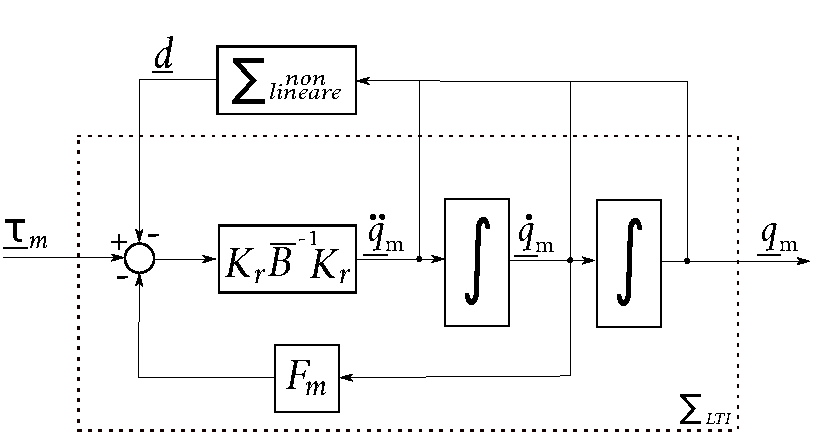
\includegraphics[scale=0.6]{controlloDecentralizzato.pdf}
	\caption{Sistema manipolatore e azionamenti.}
\end{center}
in pratica il sistema costituito dal manipolatore e dagli azionamenti si presenta come costituito da due sottosistemi:
\begin{enumerate}
	\item Il sistema con ingresso $\underline{\tau}_{\,m}$ e uscita $\underline{q}_{\,m}$ è \textbf{lineare e disaccoppiato} nel senso che ogni componente di $\underline{\tau}_{\,m}$ influenza solamente la corrispondente componente di $\underline{q}_{\,m}$.
	\item Il sistema con ingresso $\underline{q}_{\,m}$, $\underline{\dot{q}}_{\,m}$, $\underline{\ddot{q}}_{\,m}$ e uscita $\underline{d}$ è \textbf{non lineare e accoppiato} in quanto porta in conto tutti quei contributi che evidenziano come posizione e moto di ogni giunto si influenzino mutuamente con effetti non lineari di interazione.
\end{enumerate}

\paragraph{}
Il progetto della legge di controllo porta ad una struttura decentralizzata del controllore, in quanto ogni giunto è visto in maniera indipendente dagli altri. Modelliamo la parte non lineare $\underline{d}$ come ingressi non manipolabili di disturbo per gli azionamenti dei singoli giunti. 

Il controllore di giunto deve garantire elevate prestazioni in termini di forte reiezione ai disturbi e di capacità di inseguimento di traiettorie di riferimento. \emph{La struttura di controllo è basata sull'errore tra uscita desiderata e uscita effettiva, e la coppia sintetizzata dall'algoritmo di controllo per l'attuatore $i$ dipende solo dalla valutazione dell'errore associato all'uscita $i$}.

\paragraph{}
Pertanto il processo da controllare è l'azionamento del giunto $i$ controllato in tensione, corrispondente ad un sistema a un ingresso e una uscita della parte lineare e disaccoppiata, chiaramente l'interazione con gli altri giunti è descritta dalla componente $i$ del vettore $\underline{d}$, lo schema risulta il seguente

\begin{center}
	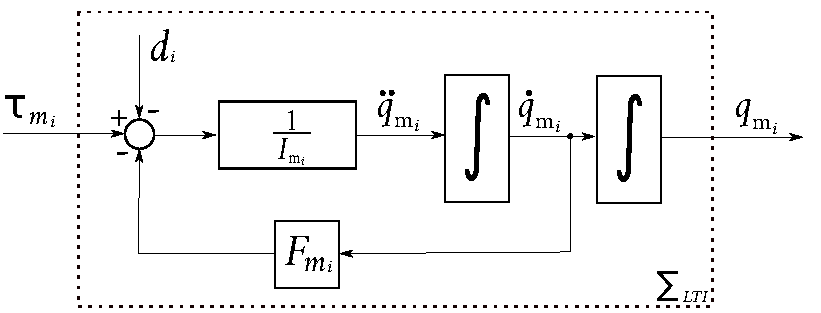
\includegraphics[scale=0.6]{decentralizzatoDisaccoppiato.pdf}
	\caption{Sistema LTI disaccoppiato.}
\end{center}

con $F_{m_i}$ la $i$-esima componente della matrice diagonale $K_r^{-T} F_v K_r^{-1}$ e $1/I_{m_i}$ la $i$-esima componente della matrice diagonale $K_r \overline{B}^{-1} K_r$.

\paragraph{}
Si utilizza in controllo decentralizzato quando:
\begin{itemize}
	\item Non sono richieste prestazioni troppo elevate in termini di precisioni del controllo $\dot{q}$, $\ddot{q}$.
	\item $K_r$ è una matrice "\emph{grossa}", ovvero $K_r^{-T} = K_r^{-1}$, quindi i rapporti di trasmissione $N_i$ elevati e filtrano la dinamica dal resto del manipolatore.
\end{itemize}


\subsection{Controllo di posizione}
Nel capitolo sugli azionamenti (capitolo 7) abbiamo esaminato la progettazione del sistema di attuazione, ovvero le modalità di cui è possibile avvalersi per controllare la velocità di rotazione dell'albero di un servomotore (elettrico). Adesso esaminiamo il problema del controllo del moto di un braccio di un generico manipolatore.

Ricorriamo a una struttura che sia in grado di determinare, in modo automatico, l'andamento temporale della grandezza scelta per controllare il motore, in modo che essa faccia eseguire al giunto interessato il movimento richiesto per consentire all'organo terminale di eseguire un determinato compito. 

\paragraph{}
La soluzione del problema è quella di considerare il moto di un giunto indipendente dal moto degli altri giunti e modellare i fenomeni di interazione come disturbi. Sia $\vartheta_r$ la traiettoria di riferimento data in ingresso come traiettoria desiderata, sia $\vartheta_m$ posizione angolare dell'asse del motore misurata da un trasduttore con costante $K_{TP}$ e sia il servomotore elettrico a corrente continua. 

Con riferimento all'azionamento pilotato in tensione di figura ($7.3$), trascurando l'induttanza $L_a$ e l'attrito $F_m$, otteniamo
\begin{equation}
	\frac{\Omega(s)}{V_a(s)} = \frac{\frac{1}{k_v}}{1+ \frac{R_a I_m}{k_v k_t} s} = \frac{k_m}{1+ T_m s}
\end{equation}

e lo schema generale di controllo dell'azionamento con retroazione di posizione è il seguente,

\begin{center}
	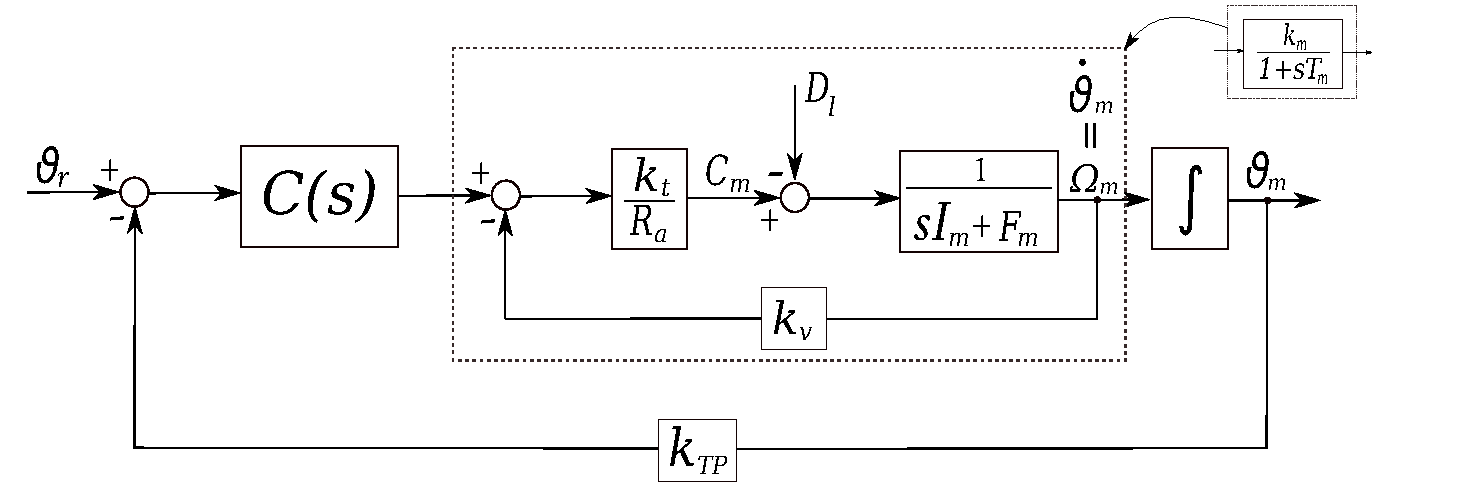
\includegraphics[scale=0.5]{controlloAzionamentoElettrico.pdf}
	\caption{Schema generale di controllo di una azionamento elettrico}
\end{center}
in pratica, il controllore posto in \emph{retroazione dinamica sull'uscita} deve garantire la reiezione dei disturbi e l'inseguimento al riferimento con minimo errore possibile. Pertanto, focalizziamoci sulla ricerca del controllore.

\paragraph{}
I requisiti del controllore che stiamo cercando sono dettati dalla riduzione degli effetti del disturbo sull'uscita. Pertanto necessitiamo di
\begin{itemize}
	\item Un alto guadagno a monte del punto di applicazione del disturbo.
	\item Un'azione integrale che annulla l'effetto della componente gravitazionale. sull'uscita.
\end{itemize}
questi requisiti suggeriscono di impiegare sulla linea di azione diretta un controllore \emph{proporzionale-integrale} (PI). Per migliorare le \emph{prestazioni dinamiche}, ovvero, ridurre ulteriormente gli effetti del disturbo, conviene realizzare il controllore come una cascata di azioni elementari e la chiusura di anelli locali di retroazione che contengano al loro interno il punto di applicazione del disturbo.

La soluzione più completa si ottiene con la chiusura di anelli interni di posizione, velocità e accelerazione,
\begin{center}
	\includegraphics[scale=0.3]{schemaGeneraleControlloPosizione.pdf}
	\caption{Struttura generale di controllo indipendente al giunto.}
\end{center}
esaminando lo schema otteniamo:
\begin{itemize}
	\item $C_{P}(s)$, $C_{V}(s)$, $C_{A}(s)$ sono i controllori di \emph{posizione}, \emph{velocità} e \emph{accelerazione}.
	\item $k_{TP}$, $k_{TV}$, $k_{TA}$ sono le rispettive costanti di trasduzione di posizione, velocità e accelerazione.
	\item Il disturbo $D$ è scalato di una costante $R_a/k_t$ (vedi riduzione a blocchi nelle appendici)
\end{itemize} 
infine notiamo l'ingresso di riferimento $\vartheta_r$ è legata all'uscita desiderata $\vartheta_{md}$ attraverso la relazione $\vartheta_r = k_{TP} \vartheta_{md}$, illustrata di seguito
\begin{center}
	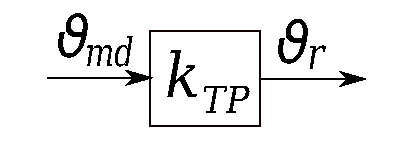
\includegraphics[scale=0.4]{trasduttoreIniziale.pdf}
	\caption{Legame tra \emph{riferimento} e \emph{uscita desiderata}.}
\end{center}
si considerano \emph{tre} casi di studio che si distinguono tra loro per il numero di cicli di retroazione attivati.

\subsubsection{\underline{Retroazione di Posizione:}}
In questo caso l'azione di controllo è caratterizzata da 
\begin{equation*}
	C_P(s) = K_P \frac{1+sT_P}{s} \qquad C_V(s) = 1 \qquad C_A(s) = 1 
\end{equation*}
con $k_{TV} = k_{TA} = 0$ la struttura generale mostrata in ($9.6$) diventa
\begin{center}
	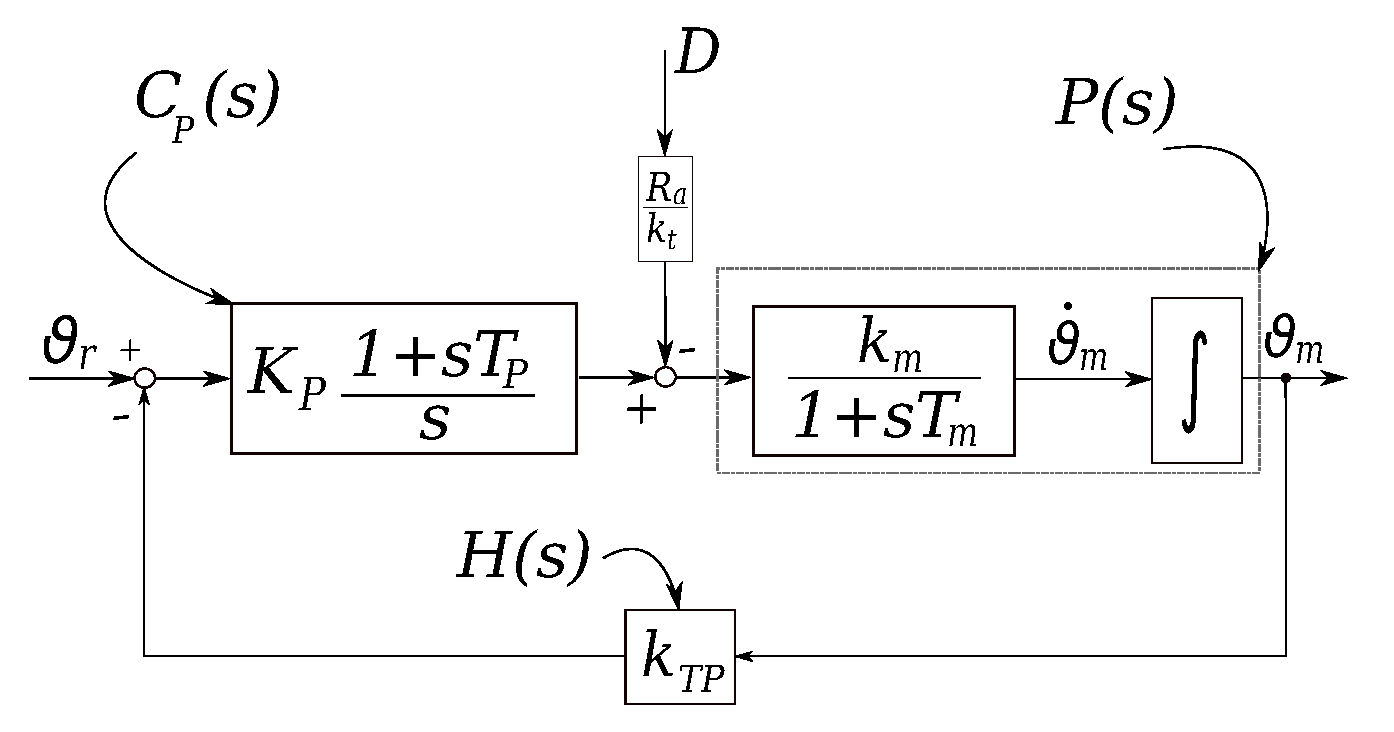
\includegraphics[scale=0.35]{schemaPos.pdf}
	\caption{Schema di controllo con retroazione di posizione.}
\end{center}
con $P(s)$ l'impianto da controllare, $H(s)$ la retroazione e la coppia $(K_P, T_P)$ rappresenta i \emph{parametri del controllore}.

La \emph{f.d.t.} ingresso-uscita in anello chiuso vale
\begin{equation}
	\frac{\vartheta_m(s)}{\vartheta_r(s)} = \frac{\frac{1}{k_{TP}}}{1+\frac{s^2(1+sT_m)}{k_mK_pk_{TP}(1+sT_P)}}
\end{equation}

La \emph{f.d.t.} disturbo-uscita vale
\begin{equation}
	\frac{\vartheta_m(s)}{D(s)} = - \frac{\frac{sR_a}{k_tK_Pk_{TP}(1+sT_P)}}{1+\frac{s^2(1+sT_m)}{k_mK_Pk_{TP}(1+sT_P)}}
\end{equation}
notiamo che l'azione integrale manda a $0$ il disturbo, infatti usando il \emph{TVF} otteniamo
\begin{equation*}
	\lim_{t \rightarrow \infty} \vartheta(t) = \lim_{s \rightarrow 0} s \vartheta(s) = \lim_{s \rightarrow 0} - \frac{R_a}{k_t} \frac{1}{k_{TP}K_P} \Bigl( s \frac{s}{(\cdots)} \frac{D}{s} \Bigr) = 0
\end{equation*} 
e se non è presente l'azione integrale si ottiene 
\begin{equation*}
	\lim_{t \rightarrow \infty} \vartheta(t) = \lim_{s \rightarrow 0} s \vartheta(s) = \lim_{s \rightarrow 0}  - \frac{R_a}{k_t} \frac{D}{\underbrace{(k_{TP}K_P)}_{X_R}} \neq 0
\end{equation*}
notiamo che il termine $X_R = k_{TP}K_P$ è il \emph{fattore di reiezione del disturbo} determinato dal guadagno $K_P$, ovvero il fattore di riduzione del disturbo. 

\paragraph{}
Definiamo la dinamica dell'azionamento attraverso l'uso del luogo delle radici (le regole per determinarlo sono nell'Appendice $B$) esaminando la funzione ad anello $L(s)$ in dipendenza della scelta del parametro $T_P$. Otteniamo
\begin{itemize}
	\item[a)] \textbf{\underline{Se $T_P < T_m$:}} Scegliamo $T_P = \frac{T_m}{2}$, lo zero è $\frac{-1}{T_P}=\frac{-2}{T_m}$, i poli sono $\lbrace 0, 0, \frac{-1}{T_m} \rbrace$. L'eccesso poli zeri è $n-m=3-1=2$, le direzioni degli asintoti sono: $\frac{\pi}{2}$, $\frac{3 \pi}{2}$ e il punto di incontro degli asintoti è $\frac{1}{2 T_m}$. Pertanto risulta che vi saranno sempre coppie di poli con pare reale maggiore di zero e quindi il sistema è instabile.
	\item[b)] \textbf{\underline{Se $T_P > T_m$:}} Scegliamo $T_P = 2T_m$, lo zero è $\frac{-1}{T_P}=\frac{-2}{T_m}$, i poli sono $\lbrace 0, 0, \frac{-1}{T_m} \rbrace$. L'eccesso poli zeri è $n-m=3-1=2$, il punto di incontro degli asintoti è $\frac{-1}{4 T_m}$. Pertanto risulta che il sistema è stabile perché i tre poli stanno tutti nel semipiano con la parte reale negativa. Ma vi è un problema, lo smorzamento dei poli dominanti (quelli più vicini all'asse immaginario, ovvero i più lenti) è insoddisfacente, in pratica, vi è una sovraelongazione.
	\item[c)] \textbf{\underline{Se $T_P \gg T_m$:}} Scegliamo $T_P = 10 T_m$, pertanto il punto di incontro degli asintoti è $\frac{-9}{20 T_m}$. Con questa scelta riesco a trovare tre poli con smorzamento unitario, pertanto il polo dominante è $ \simeq \frac{-1}{T_P}$
\end{itemize}

\begin{center}
	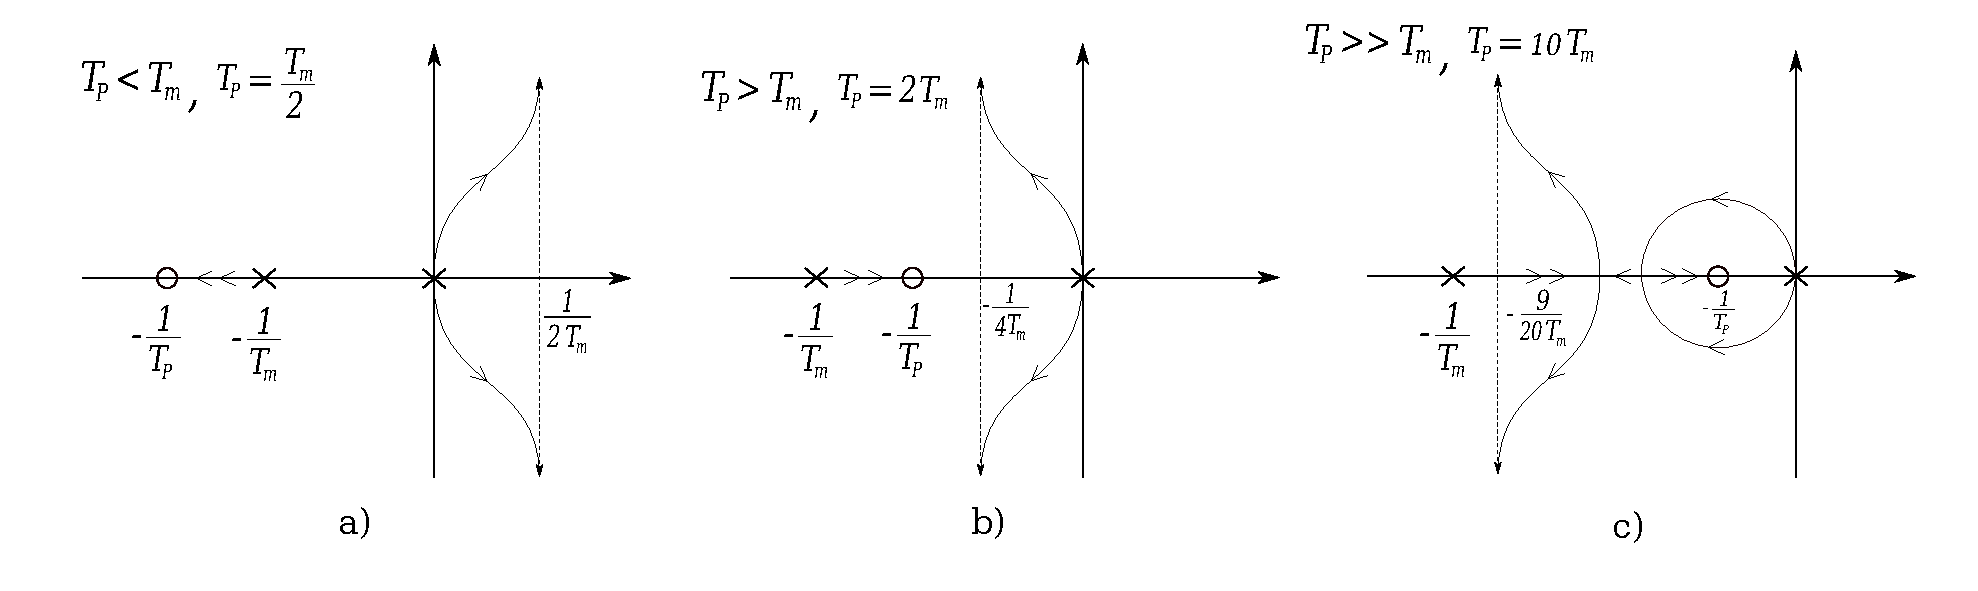
\includegraphics[scale=0.45]{rlocusPos.pdf}
	\caption{Luogo delle radici per lo schema di controllo con retroazione di posizione.}
\end{center}

\paragraph{}
La \emph{f.d.t.} ingresso-uscita nella ($9.7$) può essere espressa nella forma
\begin{equation}
	W(s) = \frac{\frac{1}{k_{TP}} (1+sT_P)}{\Bigl( 1 + \frac{2\zeta s}{\omega_n} + \frac{s^2}{\omega_n^2} \Bigr)(1+s\tau)} 
\end{equation}
dove $\omega_n$ e $\zeta$ sono rispettivamente la pulsazione naturale e il coefficiente di smorzamento della coppia di poli complessi coniugati e $-1/\tau$ è il polo reale.

Definiamo tempo di reiezione del disturbo per disturbi costanti $T_R$, come
\begin{equation}
	T_R = \max \Bigl\lbrace T_P, \frac{1}{\zeta \omega_n} \Bigr\rbrace
\end{equation}
con $\tau \approx T_P$.

\subsubsection{\underline{Retroazione di Posizione e Velocità:}}
In questo caso l'azione di controllo è caratterizzata da 
\begin{equation*}
	C_P(s) = K_P  \qquad C_V(s) = K_V \frac{1+sT_V}{s} \qquad C_A(s) = 1 
\end{equation*}
con $k_{TA} = 0$ la struttura generale mostrata in ($9.6$) diventa
\begin{center}
	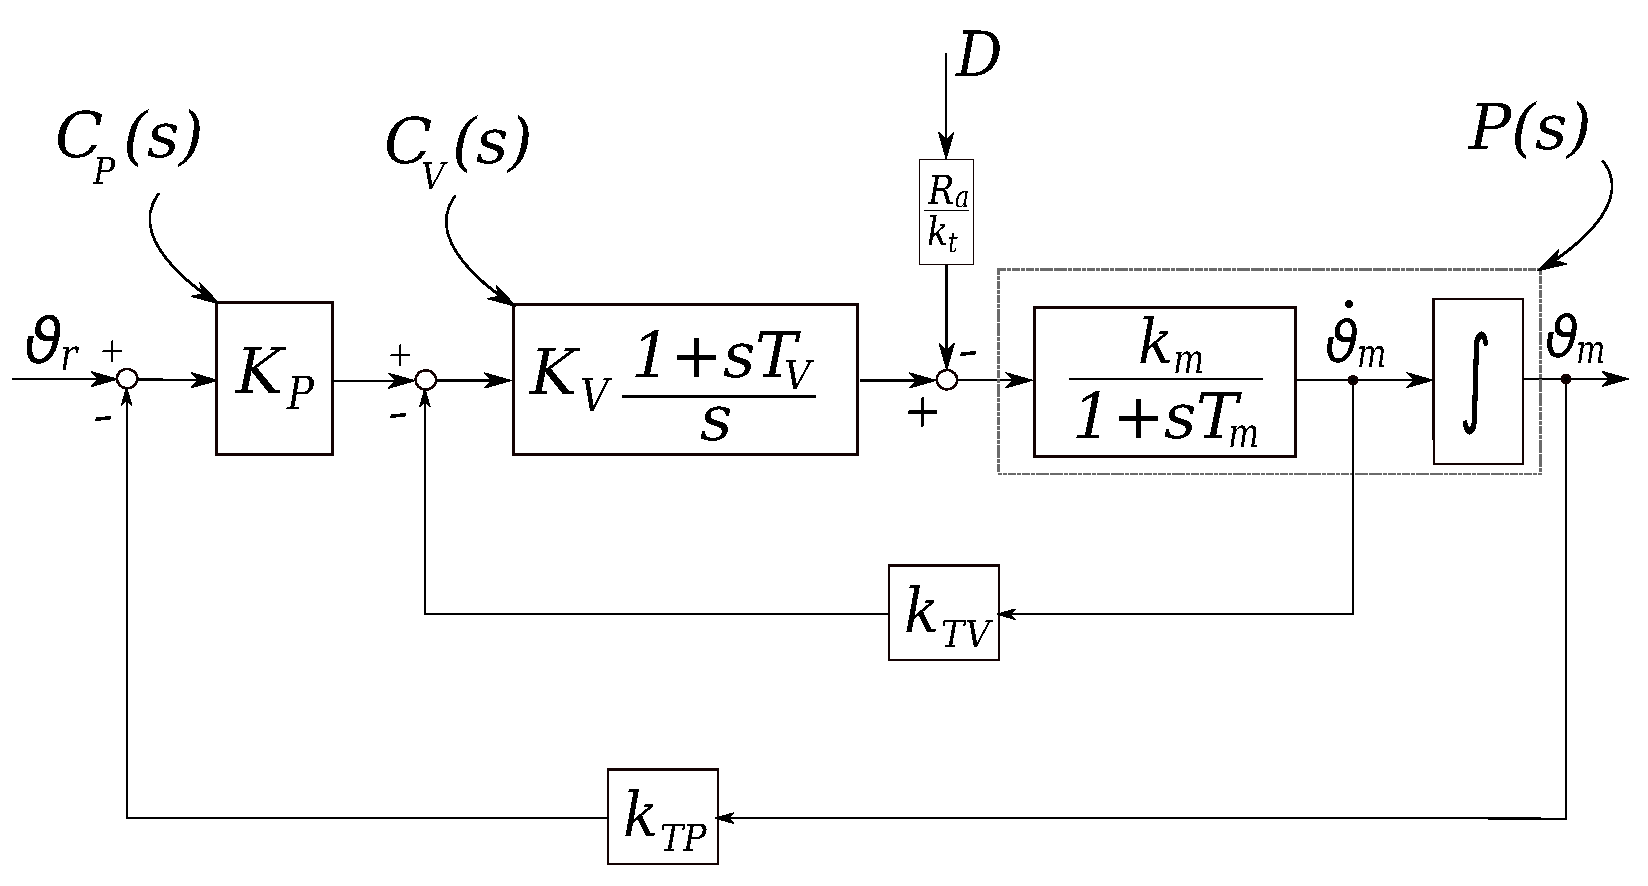
\includegraphics[scale=0.35]{schemaPosVel.pdf}
	\caption{Schema di controllo con retroazione di posizione e velocità.}
\end{center}
con $(K_P, K_V, T_V)$ \emph{parametri di progetto}. 

La \emph{f.d.t.} del ramo di azione diretta vale
\begin{equation}
	G(s) = \frac{k_m K_P K_V (1+sT_V)}{s^2(1+sT_m)}
\end{equation}
e quella del ramo di retroazione vale
\begin{equation}
	H(s) = k_{TP} \Bigl( 1+s\frac{k_{TV}}{K_Pk_{TP}} \Bigr)
\end{equation}
ponendo $T_V = T_m$ cancelliamo il polo reale del motore $s = -\frac{1}{T_m}$ con il polo reale $s = -\frac{1}{T_V}$.

\paragraph{}
La \emph{f.d.t.} ingresso-uscita in anello chiuso vale
\begin{equation}
	\frac{\vartheta_m(s)}{\vartheta_r(s)} = \frac{\frac{1}{k_{TP}}}{1+ \frac{sk_{TV}}{K_Pk_{TP}}+\frac{s^2}{k_mK_Pk_{TP}K_V}}
\end{equation}
equivalentemente 
\begin{equation}
	W(s) = \frac{\frac{1}{k_{TP}}}{1+2\frac{\zeta s}{\omega_n} + \frac{s^2}{\omega_n^2}}
\end{equation}
supponendo $\zeta$ e $\omega_n$ assegnati, si ottengono le seguenti relazioni di progetto
\begin{equation}
	\begin{cases}
		K_Vk_{TV} = \frac{2 \zeta \omega_n}{k_m} \\
		K_Pk_{TP}K_V = \frac{\omega_n^2}{k_m} 
	\end{cases}
\end{equation}

\paragraph{}
La \emph{f.d.t.} disturbo-uscita vale
\begin{equation}
	\frac{\vartheta_m(s)}{D(s)} = - \frac{\frac{s R_a}{k_tK_Pk_{TP}K_V(1+sT_m)}}{1+\frac{sk_{TV}}{K_Pk_{TP}}+\frac{s^2}{k_mK_Pk_{TP}K_V}}
\end{equation}
pertanto, il \emph{fattore di reiezione del disturbo} sull'uscita è pari a $X_R = K_P k_{TP}K_V$.

\paragraph{}
Esaminiamo il luogo delle radici, considerando
\begin{equation}
	L(s) = \frac{K_P K_V k_m k_{TP}}{s^2} \Bigr( 1 + \frac{k_{TV}s}{K_P k_{TP}} \Bigl)
\end{equation}
l'incremento del guadagno di posizione $K_P$ consente di posizionare i poli del sistema in anello chiuso in regioni del piano complesso caratterizzate da elevati valori assoluti della parte reale, definendone poi, l'allocazione puntuale con una opportuna scelta di $K_V$. Gli zeri sono $\lbrace \frac{-1}{T_V}, \frac{-k_{TP}K_P}{k_{TV}} \rbrace$, i poli invece $\lbrace 0,0,\frac{-1}{T_m} \rbrace$.
\begin{center}
	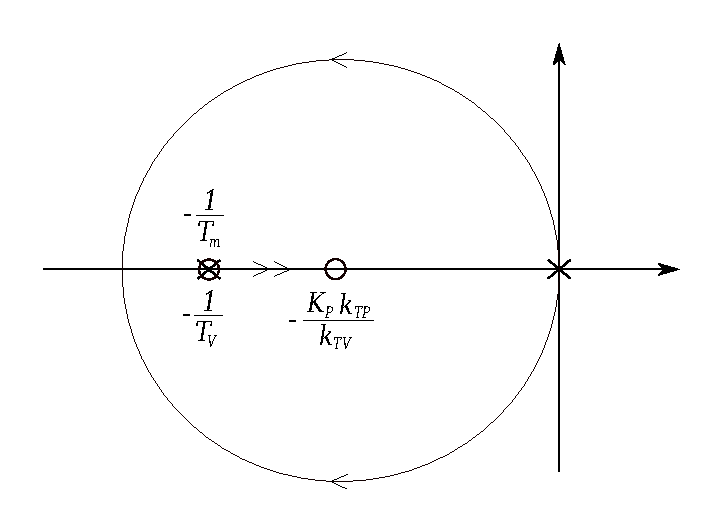
\includegraphics[scale=0.4]{rlocusPosVel.pdf}
	\caption{Luogo delle radici per lo schema con retroazione di posizione e velocità.}
\end{center} 
esaminando il \emph{tempo di recupero} $T_R$, si ha
\begin{equation}
	T_R = \max \lbrace T_m, \frac{1}{\zeta \omega_n} \rbrace 
\end{equation}
se piazzo lo zero di $H(s)$, tramite un $K_P$ più grande, a sinistra della coppia cancellata, il sistema migliora in termini di prontezza e notiamo un miglioramento rispetto alla sola retroazione di posizione, ma $T_R$ resta uguale.

\subsubsection{\underline{Retroazione di Posizione, Velocità e Accelerazione:}}
In questo caso l'azione di controllo è caratterizzata da 
\begin{equation*}
	C_P(s) = K_P  \qquad C_V(s) = K_V  \qquad C_A(s) = K_A\frac{1+sT_A}{s} 
\end{equation*}
con tutti i trasduttori $\neq 0$, la struttura generale mostrata in ($9.6$) diventa
\begin{center}
	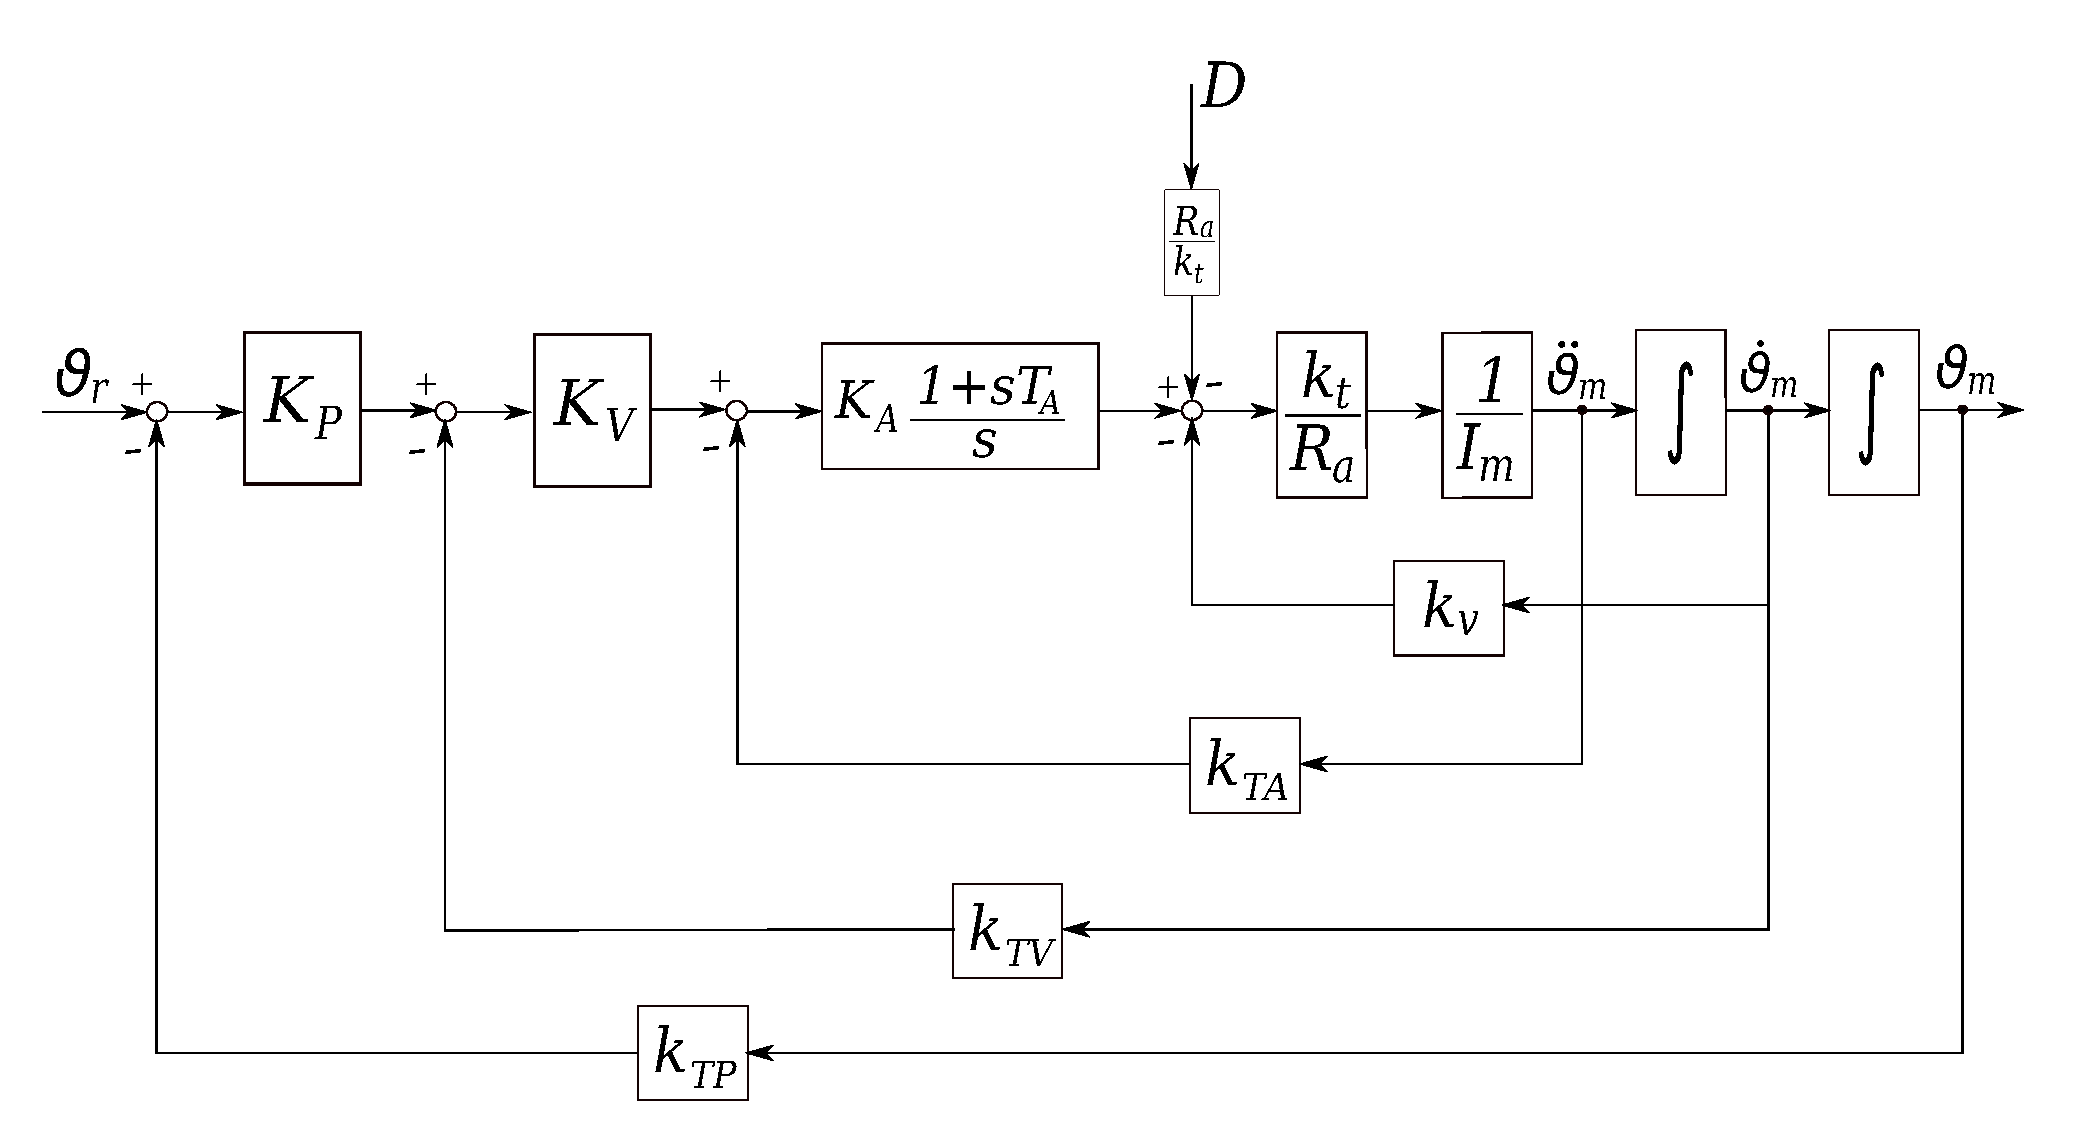
\includegraphics[scale=0.35]{schemaPosVelAcc.pdf}
	\caption{Schema di controllo con retroazione di posizione, velocità e accelerazione.}
\end{center}
con $(K_P, K_V, K_A, T_A)$ \emph{parametri di progetto}. 

La \emph{f.d.t.} del ramo di azione diretta vale 
\begin{equation*}
	G(s) = \Biggl( \frac{K_P K_V K_A (1+sT_A)}{s^2} \Biggr) \Biggl( \frac{k_m}{(1+k_mK_Ak_{TA})\Bigl( 1+\frac{sT_m(1+k_mK_Ak_{TA}\frac{T_A}{T_m})}{(1+k_mK_Ak_{TA})} \Bigr)} \Biggr)
\end{equation*}

La \emph{f.d.t.} del ramo di retroazione vale
\begin{equation}
	H(s) = k_{TP}\Bigl( 1+ \frac{sk_{TV}}{K_Pk_{TP}} \Bigr)
\end{equation}

\paragraph{}
Abbiamo due modi per cancellare il polo del motore 
\begin{itemize}
	\item In maniera diretta, $T_A = T_m$, in questo caso ottengo $T_R = T_m = T_A$ e mi riconduco al caso di retroazione di posizione e velocità.
	\item In maniera indiretta, ponendo
	\begin{equation}
		k_mK_Ak_{TA}T_A \gg T_m \qquad k_mK_Ak_{TA} \gg 1
	\end{equation}
	così facendo la costante $T_A$ rimane libera e posso sceglierla $< T_m$.
\end{itemize}

\paragraph{}
Facendo la seconda scelta, consideriamo 
\begin{equation}
	L(s) = \Bigl( \frac{k_{TV}K_VK_Ak_m}{1+k_{TA}K_Ak_m} \Bigr) \Bigl( \frac{s+\frac{k_{TP} K_P}{k_{TV}}}{s^2} \Bigr)
\end{equation}
e il luogo delle radici risulta,
\begin{center}
	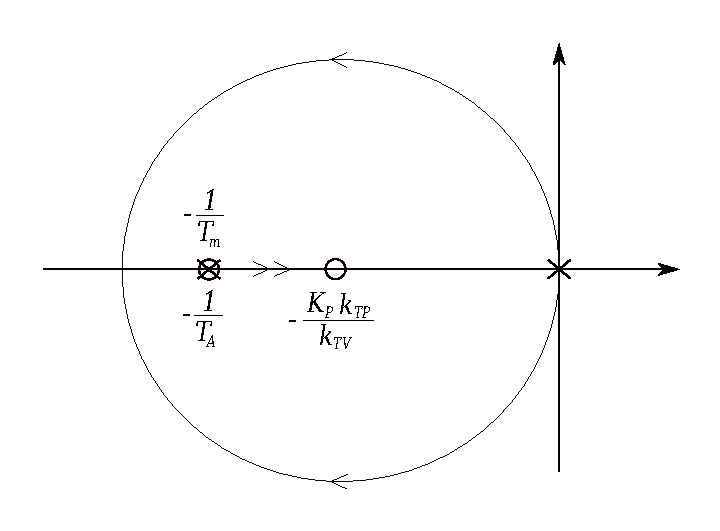
\includegraphics[scale=0.4]{rlocusPosVelAcc.pdf}
	\caption{Luogo delle radici per il controllo con retroazione di posizione, velocità e accelerazione.}
\end{center}

\paragraph{}
La \emph{f.d.t.} ingresso-uscita in anello chiuso è
\begin{equation}
	\frac{\vartheta_m(s)}{\vartheta_r(s)} = \frac{\frac{1}{k_{TP}}}{1+\frac{sk_{TV}}{K_Pk_{TP}}+\frac{s^2(1+k_mKAk_{TA})}{k_mK_Pk_{TP}K_VK_A}}
\end{equation}

La \emph{f.d.t.} disturbo-uscita è
\begin{equation}
	\frac{\vartheta_m(s)}{D(s)} = -\frac{\frac{s R_a}{k_tK_Pk_{TP}K_VK_A(1+sT_A)}}{1+\frac{sk_{TV}}{K_Pk_{TP}}+\frac{s^2(1+k_mK_Ak_{TA})}{k_mK_Pk_{TP}K_VK_A}}
\end{equation}

Pertanto, il \emph{fattore di riduzione} è il seguente
\begin{equation}
	X_R = K_Pk_{TP}K_VK_A
\end{equation}
e il \emph{tempo di recupero} è caratterizzato da
\begin{equation}
	T_R = \max \lbrace T_A, \frac{1}{\zeta \omega_n} \rbrace
\end{equation}
con $T_A$ controllabile.

\paragraph{}
Con riferimento alla funzione tipica del secondo ordine $W(s)$ riportata in ($9.14$), otteniamo con analogia alle relazioni in ($9.15$), le seguenti equazioni,
\begin{equation}
	\begin{cases}
		\frac{2K_Pk_{TP}}{k_{TV}} = \frac{\omega_n}{\zeta} \\
		k_mK_Ak_{TA} = \frac{k_mX_R}{\omega_n^2} - 1\\
		K_Pk_{TP}K_VK_A = X_R
	\end{cases}
\end{equation}
notiamo che la retroazione di accelerazione consente di ottenere, un qualsiasi comportamento dinamico desiderato e inoltre rispetto ai casi precedenti, consente di prefissare il fattore di riduzione degli effetti indotti dal disturbo.

\newpage

\subsection{Misura di grandezze retroazionate} 
Le tre soluzioni di controllo fino adesso illustrate trascurano un problema fondamentale che si presenta nella pratica, ovvero, la misura delle grandezze da retroazionare. Infatti, non vi è alcun problema nel misurare posizione e velocità, mentre una misura diretta dell'accelerazione non è disponibile e risulta onerosa da ottenere. 

Nel retroazionare l'accelerazione nella terza soluzione illustrata nella Figura 9.12, possiamo ricorrere a una misura indiretta, ovvero, ricostruiamo la grandezza \emph{accelerazione} con un \textit{\textbf{filtro del primo ordine}}.
\begin{center}
	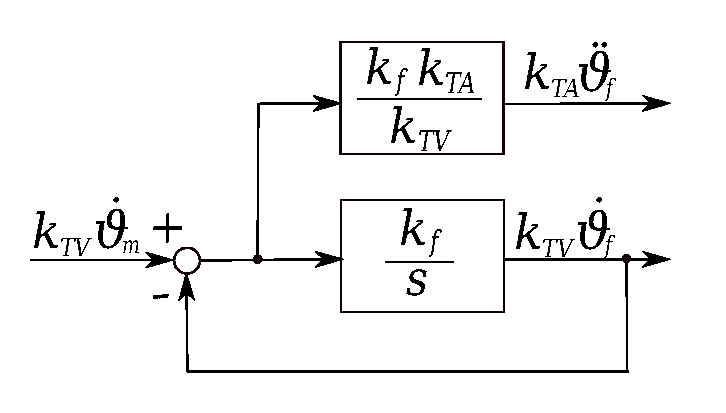
\includegraphics[scale=0.4]{filtroDerivata.pdf}
	\caption{Filtro ricostruttore della \emph{derivata}.}
\end{center}

Il filtro ricostruisce l'operazione di \emph{derivazione} ed è caratterizzato da una banda passante a 3 dB $\omega_{3f} = k_f$. Scegliendo tale banda sufficientemente ampia, gli effetti dei ritardi indotti nella misura possono ritenersi trascurabili e quindi è lecito utilizzare come grandezza da retroazionare l'uscita in accelerazione del filtro.

Posso ricorrere alla \emph{tecnica del filtraggio} anche se ho solo la posizione come grandezza disponibile, infatti, ricorrendo ad un filtro del \emph{secondo} ordine, posso ricostruire sia la velocità che l'accelerazione. Chiaramente ho più errori e difficoltà di implementazione numerica del controllore.

\subsection{Compensazione in avanti decentralizzata}
Quando si considerano azionamenti a cui sono imposte traiettorie desiderate in posizione caratterizzate da elevati valori di velocità e accelerazioni, le capacità di \textbf{inseguimento} presentate dallo schema ($9.6$) sono degradate. 

L'adozione di un'azione di \emph{compensazione in avanti decentralizzata} consente di ridurre l'errore di inseguimento a meno dell'effetto dei disturbi. I nuovi ingressi risultano,
\begin{align}
	\vartheta_r(s) = \Bigl( k_{TP} + \frac{s^2(1+sT_m)}{k_mK_p(1+sT_P)}  \Bigr) \vartheta_{md}(s) \\
	\vartheta_r(s) = \Bigl( k_{TP} + s\frac{k_{TV}}{K_P} + \frac{s^2}{k_mK_PK_V} \Bigr) \vartheta_{md}(s) \\
	\vartheta_r(s) = \Bigl( k_{TP} + s\frac{k_{TV}}{K_P} \frac{s^2(1+k_mK_Ak_{TA})}{k_mK_PK_VK_A}\Bigr) \vartheta_{md}(s)
\end{align}
in tal modo si ottiene l'inseguimento della posizione desiderata $\vartheta_{md}(s)$. I tre schemi risultanti si ottengono attraverso semplici manipolazione in catena diretta da $\vartheta_r(s)$ negli schemi 9.8, 9.10 e 9.12. Otteniamo
\begin{center}
	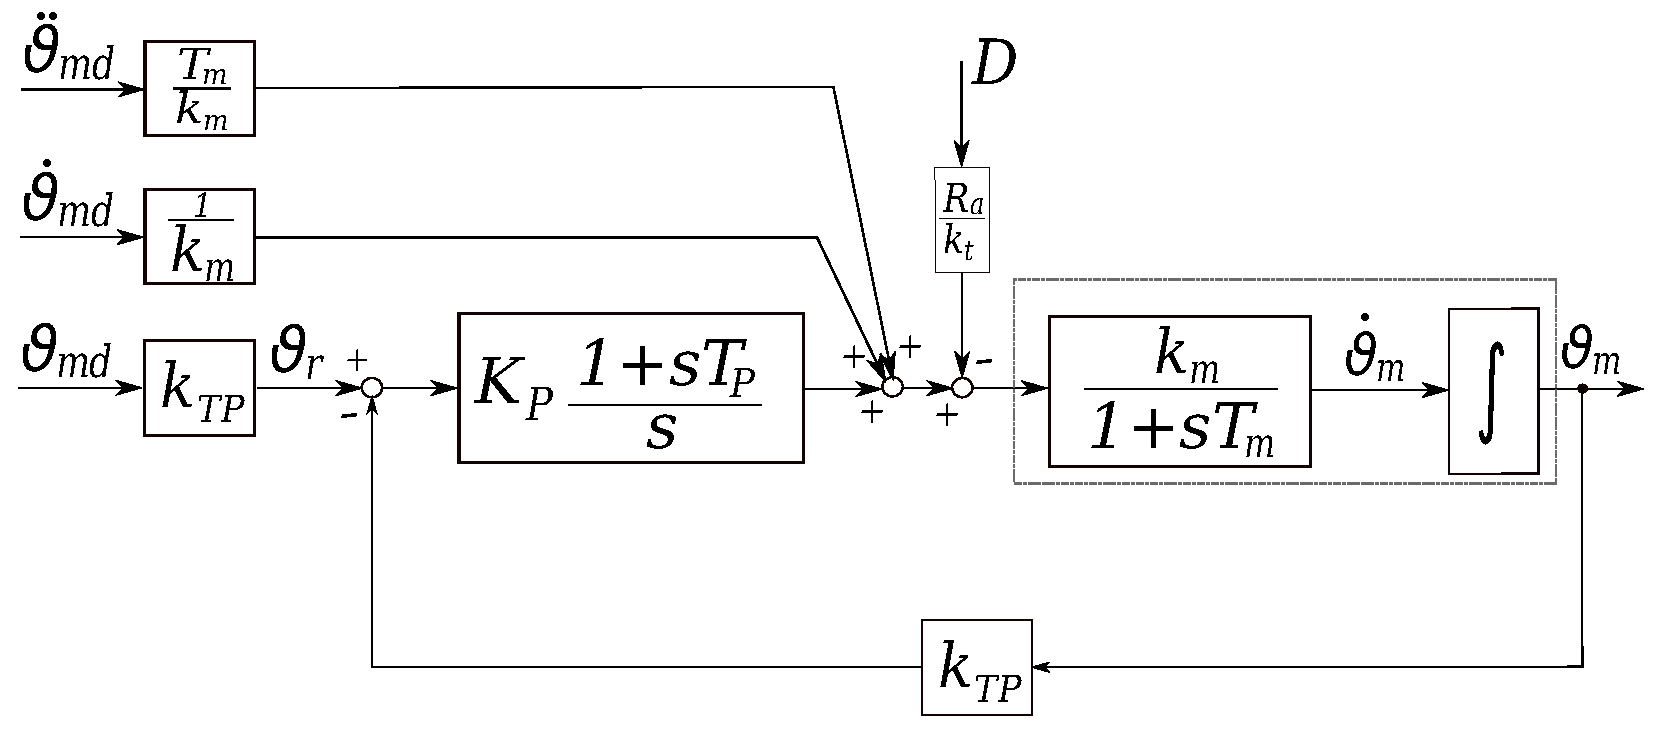
\includegraphics[scale=0.35]{compensazioneAvantiPos.pdf}
	\caption{Retroazione di posizione con compensazione in avanti decentralizzata.}
	
	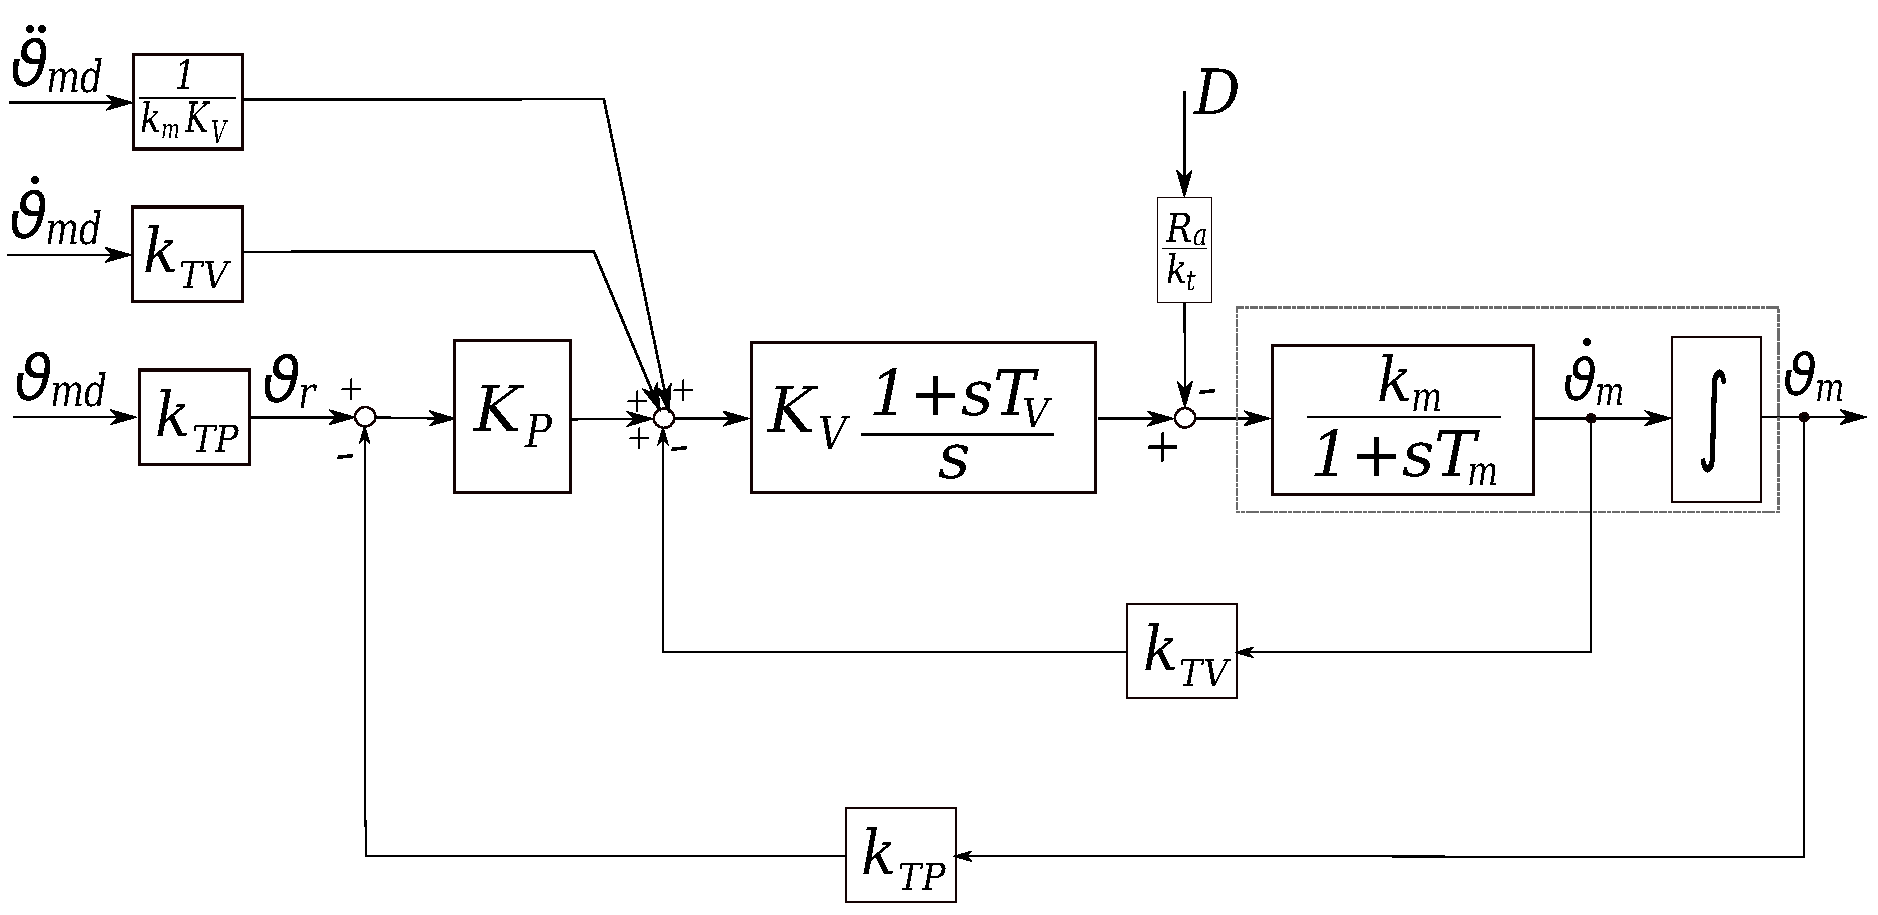
\includegraphics[scale=0.35]{compensazioneAvantiPosVel.pdf}
	\caption{Retroazione di posizione e velocità con compensazione in avanti decentralizzata.}
	
	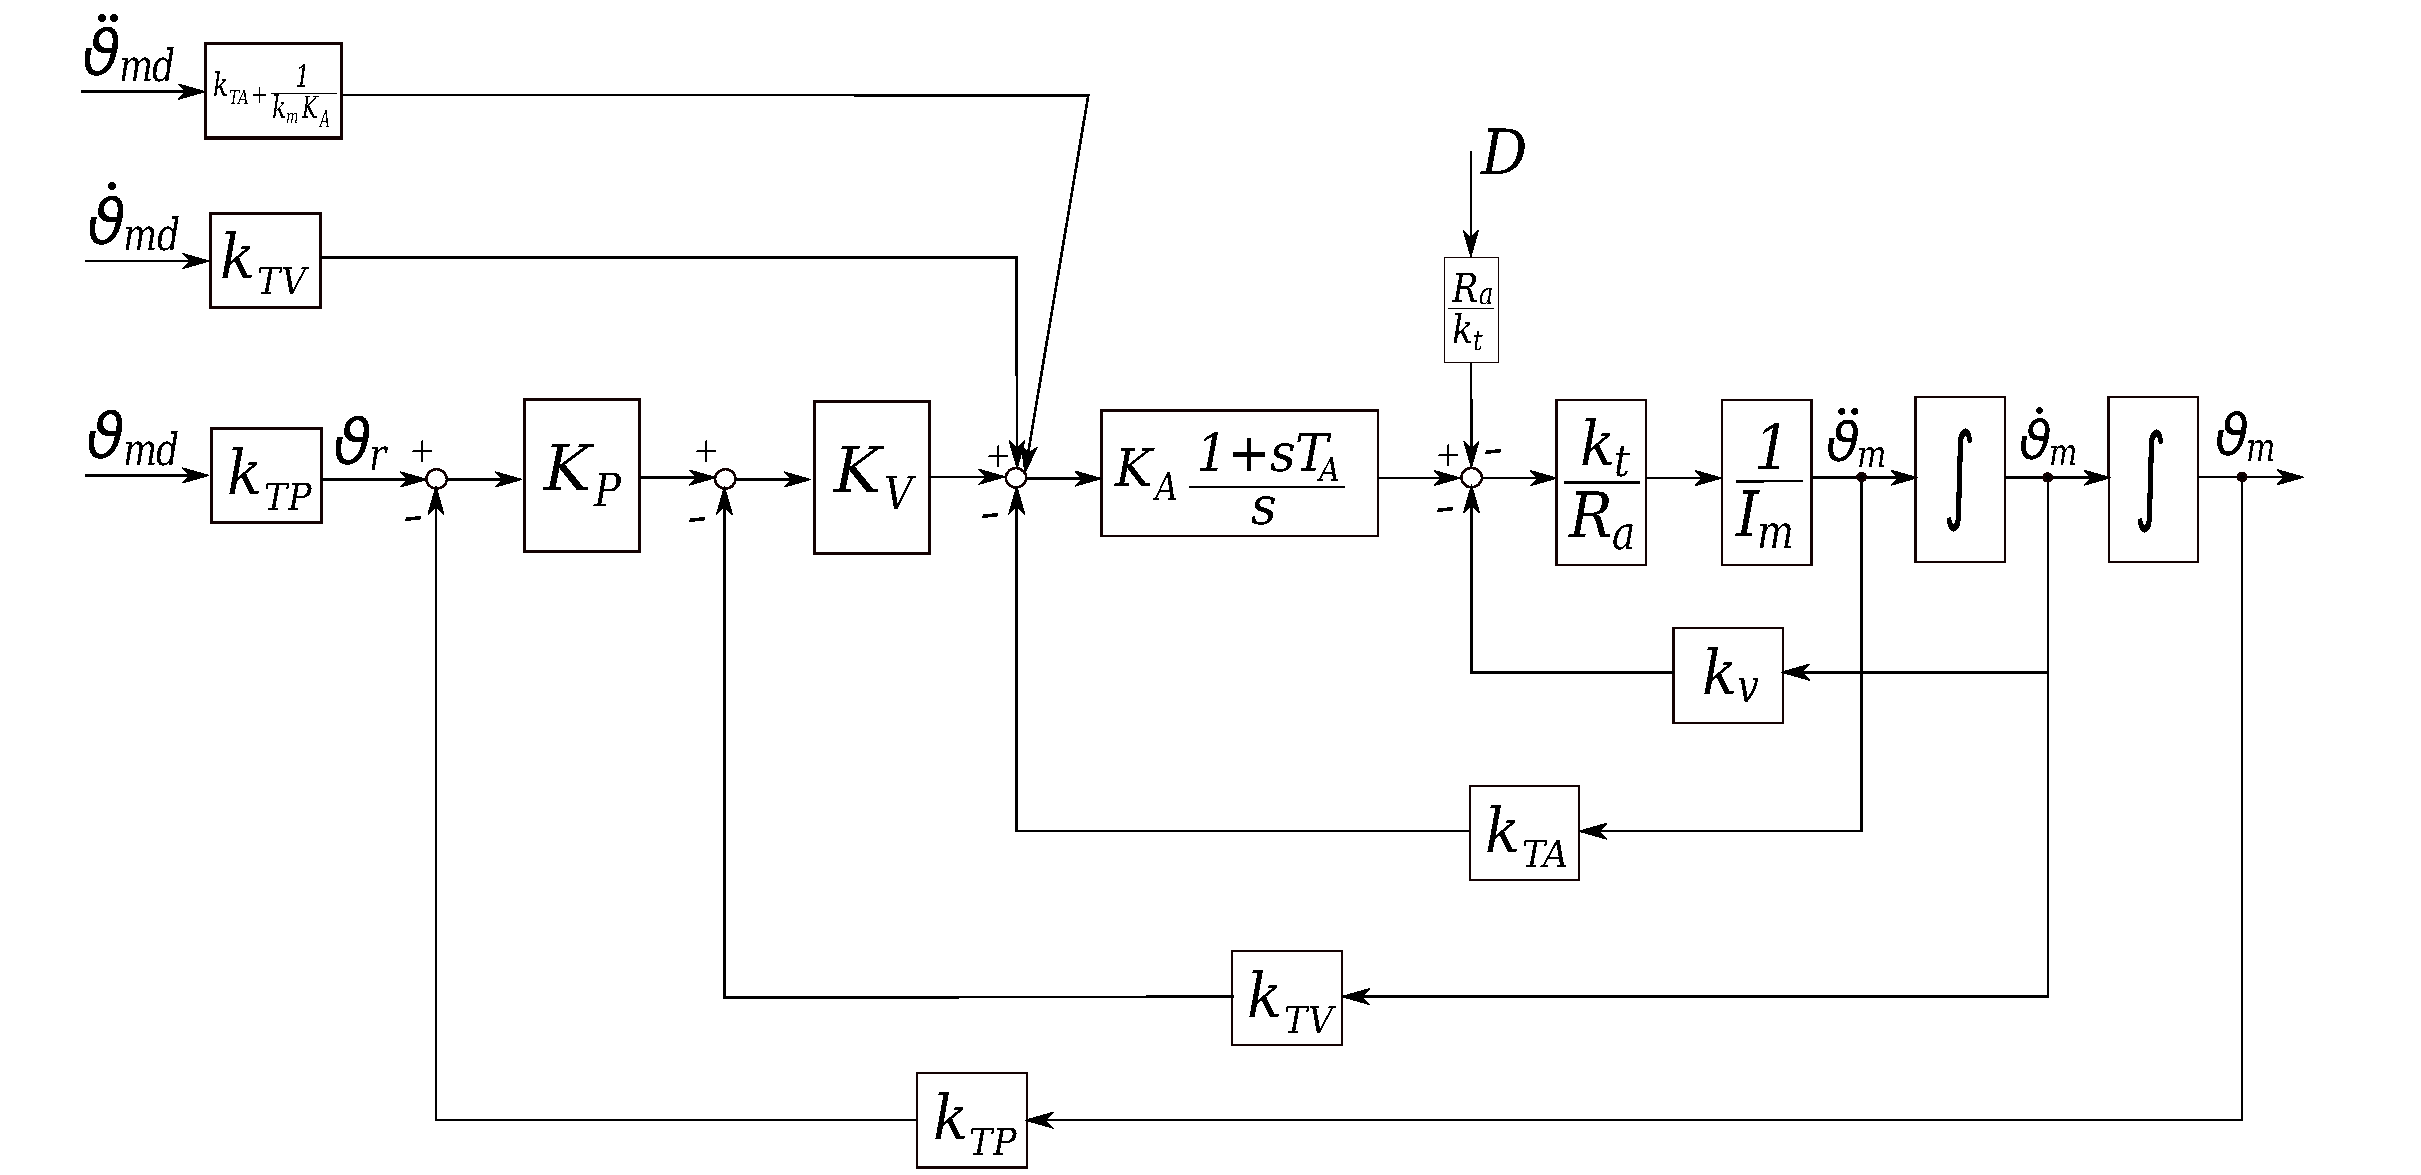
\includegraphics[scale=0.35]{compensazioneAvantiPosVelAcc.pdf}
	\caption{Retroazione di posizione, velocità e accelerazione con compensazione in avanti decentralizzata.}
\end{center}

\paragraph{}
Notiamo che al crescere del numero di anelli interni, si riduce la conoscenza del sistema di attuazione necessaria per la realizzazione dell'azione in avanti. Infatti,
\begin{itemize}
	\item Per lo schema in figura 9.15 è richiesta la conoscenza di $T_m$ e $k_m$.
	\item Per lo schema in figura 9.16 è richiesta la conoscenza di $k_m$.
	\item Per lo schema in figura 9.17 è richiesta la conoscenza di $k_m$ ma con peso ridotto.
\end{itemize}

Questa soluzione, presenta delle \emph{non linearità} intenzionali la cui funzione è quella di limitare, nei transitori, grandezze fisiche di particolare interesse. Al crescere del numero di anelli di retroazione aumenta il numero di grandezze su cui è possibile effettuare operazioni di limitazione (velocità, accelerazione e tensione del motore). 

\paragraph{}
Possiamo individuare delle \emph{strutture di controllo equivalenti} che utilizzano la sola retroazione di posizione e regolatori con azioni standard. Queste strutture hanno le stesse caratteristiche di reiezione dei disturbi e inseguimento di riferimenti, però l'eliminazione degli anelli di retroazione interni toglie la possibilità di inserire limitazioni sulla velocità e sulla accelerazione. 

Le \emph{azioni di controllo} in questi nuovi schemi hanno le seguenti \emph{equivalenze},
\begin{itemize}
	\item Retroazione di posizione $\Longleftrightarrow$ PI.
	\item Retroazione di posizione e velocità $\Longleftrightarrow$ PID.
	\item Retroazione di posizione, velocità e accelerazione $\Longleftrightarrow$ PIDD$^2$.
\end{itemize}
pertanto gli schemi equivalenti alle figure 9.15, 9.16, 9.17 sono rispettivamente
\begin{center}
	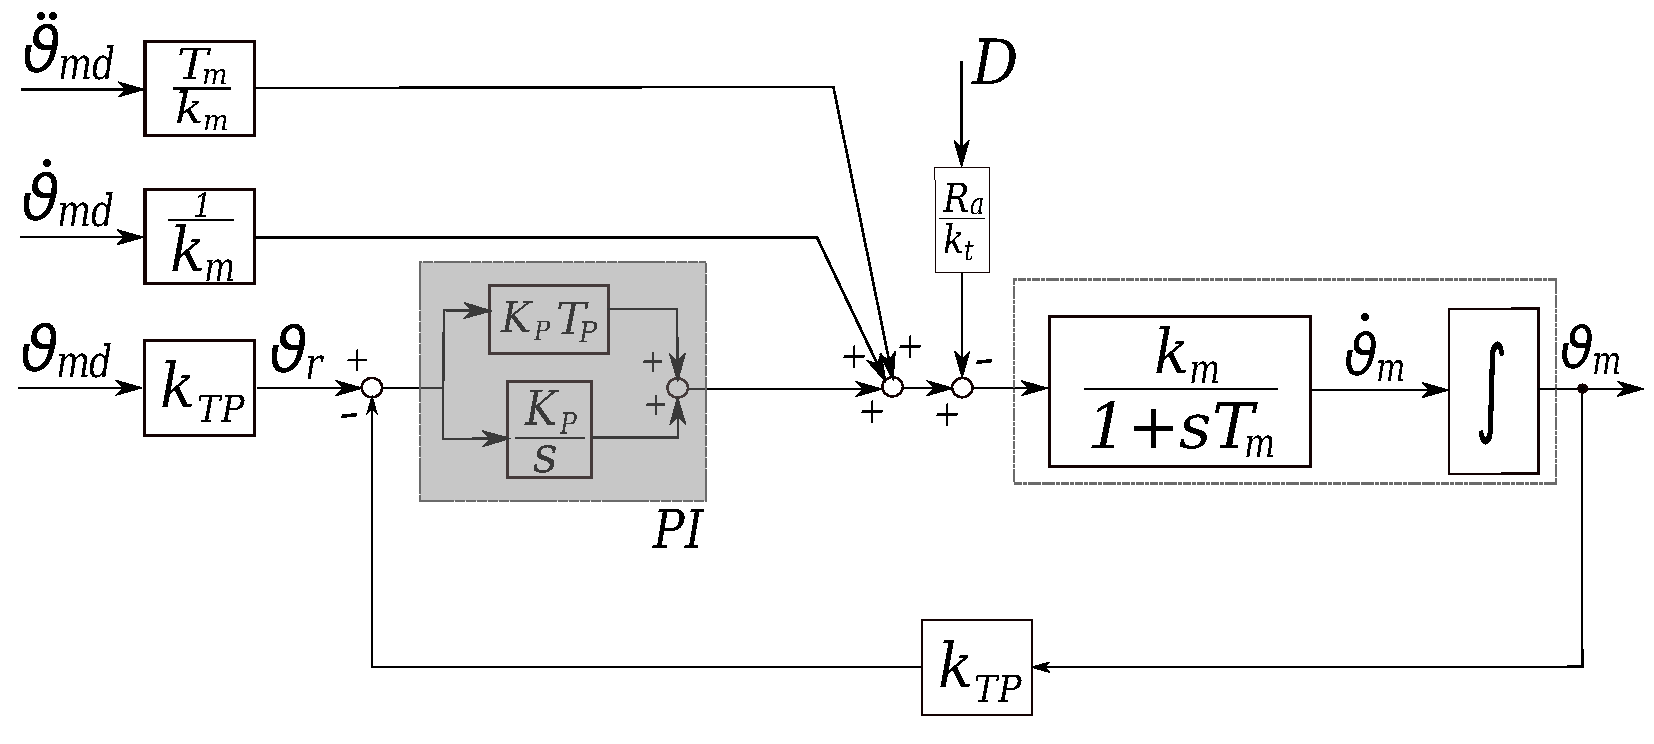
\includegraphics[scale=0.35]{PI.pdf}
	\caption{Retroazione di posizione di tipo PI, equivalente allo schema 9.15}
	
	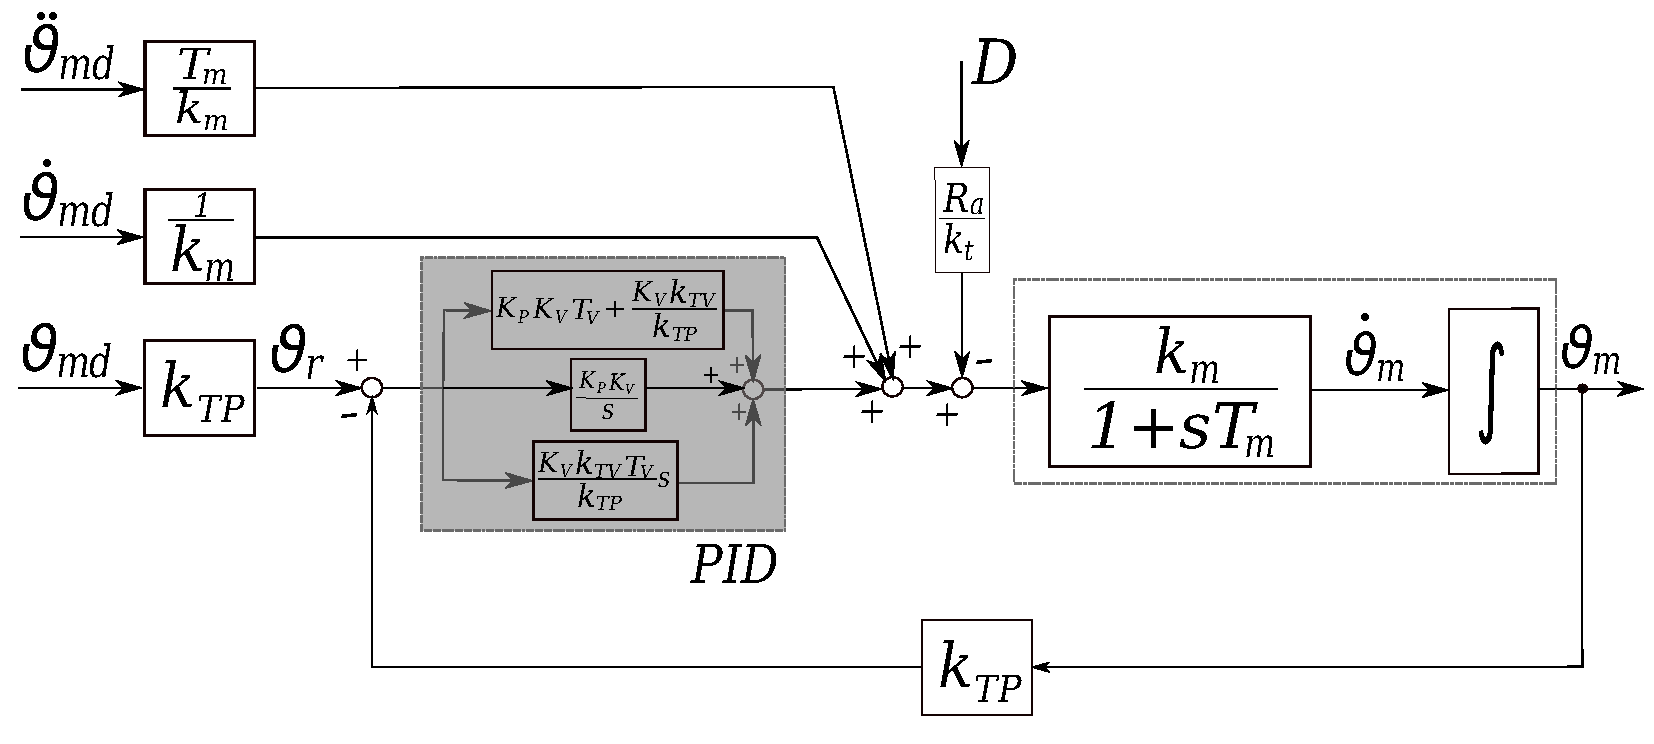
\includegraphics[scale=0.35]{PID.pdf}
	\caption{Retroazione di posizione di tipo PID, equivalente allo schema 9.16}
	
	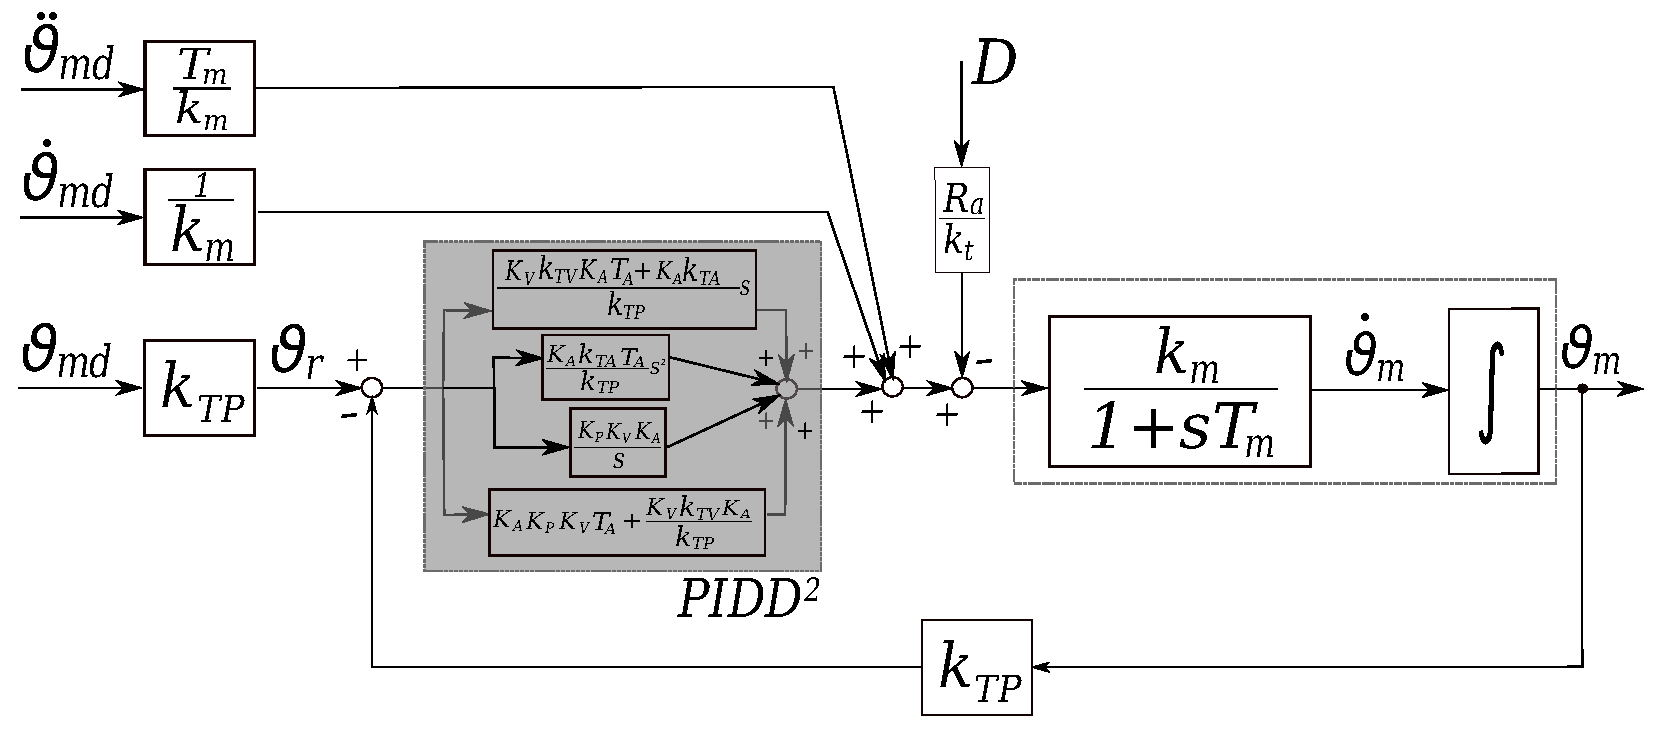
\includegraphics[scale=0.35]{PIDD.pdf}
	\caption{Retroazione di posizione di tipo PIDD$^2$, equivalente allo schema 9.17}
\end{center}
notando che queste strutture sono tutte caratterizzate dalla presenza dell'azione in avanti $(\frac{T_m}{k_m})\dot{\vartheta}_{md} + (\frac{1}{k_m}) \dot{\vartheta}_{md}$.

\subsection{Riepilogo}
Facciamo un prospetto riassuntivo del \textbf{controllo decentralizzato} visto fino adesso,
\begin{center}
	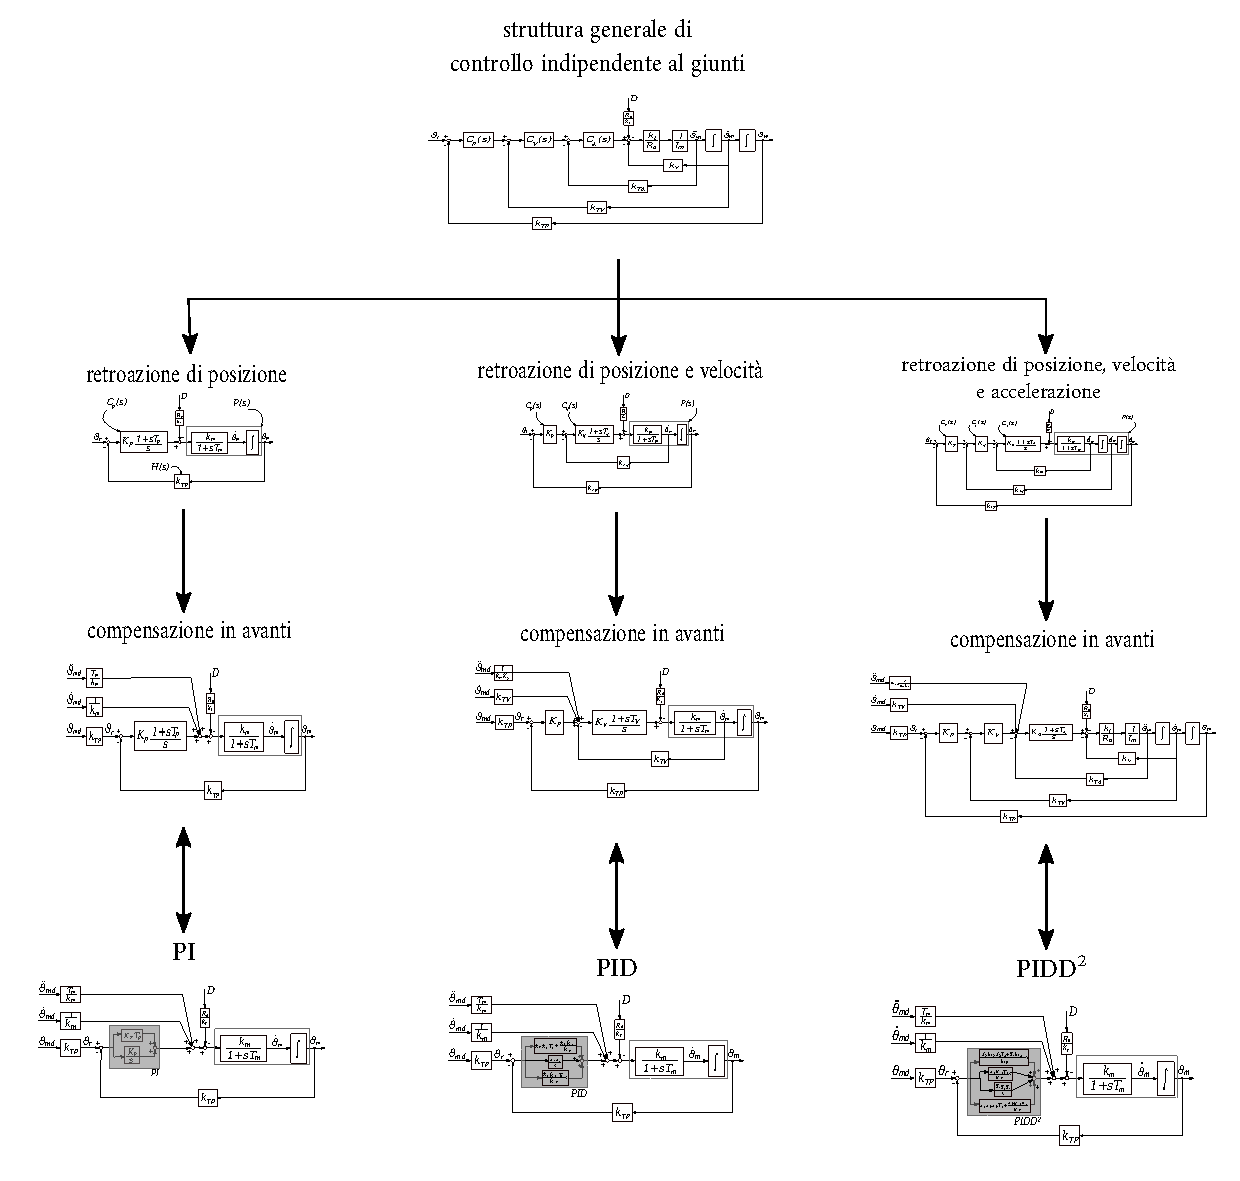
\includegraphics[scale=0.56]{riassuntoDecentralizzato.pdf}
\end{center}

\section{Controllo Centralizzato}
Fino adesso, abbiamo considerato gli effetti di interazione e accoppiamento tra i diversi giunti come \emph{cause di disturbo} agenti su ogni singolo azionamento. Quando però abbiamo un manipolatore con attuatori ad accoppiamento diretto o attuatori ad alta velocità di movimento, i termini non lineari di accoppiamento influenzano in maniera massiva le prestazioni del sistema, per cui considerare l'effetto delle componenti di $\underline{d}$ come disturbi può generare errori notevoli nell'inseguimento di traiettorie desiderate.

Pertanto, è necessario agire sulla \emph{eliminazione delle cause di disturbo} piuttosto che sulla riduzione degli \emph{effetti del disturbo}, generando delle coppie (o forze) che vadano a compensare gli effetti dell'interazione espressi dal vettore $\underline{d}$ in ($9.5$). Useremo quindi, \emph{schemi di controllo centralizzato} basati sulla conoscenza, parziale o completa, del modello dinamico del manipolatore.

\paragraph{}
\textbf{\textit{Come mostrato dal modello matematico $(9.1)$, il manipolatore non è un insieme di n sistemi disaccoppiati ma è un sistema multivariabile, con n ingressi (le coppie ai giunti) ed n uscite (le posizioni dei giunti) tra di loro interagenti con legami di tipo non lineare.}}

\paragraph{}
L'obiettivo è quello di inseguire una traiettoria $\underline{q}_{\,d}$, $\dot{\underline{q}}_{\,d}$, $\ddot{\underline{q}}_{\,d}$ con sistema di errore globalmente, asintoticamente stabile. Affrontiamo il problema della determinazione della legge $\underline{\tau}$ che assicura il soddisfacimento di prestazioni al sistema manipolatore-attuatori considerato.

\subsection{Controllo PD con compensazione di gravità}
Sia assegnata una postura costante di equilibrio con un vettore di posizione desiderate ai giunti $\underline{q}_{\,d}$. Mediante la chiusura di anelli di posizione su ogni giunto, si vuole individuare la struttura del controllore che assicuri la stabilità asintotica globale della posizione di equilibrio. Lo stato è il vettore,
\begin{equation}
	\begin{bmatrix}
		\underline{e} \\
		\underline{\dot{q}}
	\end{bmatrix}
\end{equation}
dove $\underline{e} = \underline{q}_{\,d} - \underline{q}$ rappresenta l'errore di posizione.

\paragraph{}
Utilizziamo il \emph{metodo diretto di Lyapunov} per determinare il vettore di controllo che garantisce la stabilizzazione del punto di equilibrio. Si scelga come candidata di Lyapunov, la forma quadratica definita positiva
\begin{equation}
	V(\dot{\underline{q}}, \underline{e}) = \frac{1}{2} \underline{\dot{q}}^T B(\underline{q})\underline{\dot{q}} + \frac{1}{2} \underline{e}^T K_P \underline{e} > 0 \qquad \forall\underline{\dot{q}}, \underline{e} \neq 0
\end{equation}
con $K_P \in \mathbb{R}^{n \times n}$ simmetrica e definita positiva. Una interpretazione energetica evidenzia un primo termine che rappresenta l'energia cinetica della struttura e un secondo termine che rappresenta l'energia elastica di un sistema di molle con rigidità $K_P$ realizzato dagli $n$ anelli di retroazione di posizione.

Derivando la candidata e ricordando che $\underline{q}_{\,d}$ è costante, otteniamo,
\begin{equation}
	\dot{V} = \underline{\dot{q}}^T B(\underline{q}) \ddot{\underline{q}} + \frac{1}{2}\underline{\dot{q}}^T \dot{B}(\underline{q}) \underline{\dot{q}} + \underline{e}^T K_P \underline{\dot{e}} = \underline{\dot{q}}^T \Bigl( -K_P \underline{e} + B \underline{\ddot{q}} + \frac{1}{2} \dot{B}\underline{\dot{q}} \Bigr)
\end{equation}
adesso consideriamo
\begin{equation}
	\ddot{q} = B^{-1}(\underline{q}) \Bigl( \underline{\tau} - C(\underline{q}, \underline{\dot{q}})\underline{\dot{q}} - F_v \underline{\dot{q}} - \underline{g}(\underline{q}) \Bigr)
\end{equation}
e sostituendo alla ($9.32$),
\begin{equation}
	\dot{V} = \underline{\dot{q}}^T \Bigl( -K_P \underline{e} + \underline{\tau} - C \underline{\dot{q}} - F_v \underline{\dot{q}} - \underline{g}(\underline{q}) + \frac{1}{2} \dot{B} \underline{\dot{q}} \Bigr)
\end{equation}
e adesso ricordando che la matrice $\dot{B} - 2C$ è antisimmetrica, la proprietà che ci viene in aiuto per questa dimostrazione di stabilità è
\begin{equation}
	\underline{\dot{q}}^T \Bigl( \frac{1}{2} \dot{B} - C \Bigr) \underline{\dot{q}} = 0
\end{equation}
adesso troviamo un $\underline{\tau}$ tale che $\dot{V} < 0$,
\begin{itemize}
	\item Mettiamo un termine $K_P \underline{e}$ per neutralizzare $- K_P \underline{e}$.
	\item Mettiamo un termine $\underline{g}(\underline{q})$ per compensare la gravità $-\underline{g}(\underline{q})$.
	\item Mettiamo un termine che renda ancora più negativo $\dot{V}$, ovvero, una retroazione tachimetrica $- K_D \underline{\dot{q}}$ con $K_D$ definita positiva.
\end{itemize}
otteniamo la seguente legge di controllo,
\begin{equation}
	\underline{\tau} = K_P \underline{e} - K_D \underline{\dot{q}} + \underline{g}(\underline{q})
\end{equation}
e riscrivendo la ($9.34$) otteniamo
\begin{equation}
	\dot{V} = - \underline{\dot{q}}^T (F_v + K_D)\underline{\dot{q}}
\end{equation}
che evidenzia quanto il termine derivativo $K_D$ renda il sistema più pronto.

\paragraph{}
La dinamica del sistema controllato con la legge ($9.36$) è espressa da
\begin{equation}
	B(\underline{q})\underline{\ddot{q}} + C(\underline{q}, \underline{\dot{q}})\underline{\dot{q}} + \underline{g}(\underline{q}) = \underline{g}(\underline{q}) + K_P \underline{e} - K_D \underline{\dot{q}}
\end{equation}
e all'equilibrio ($\underline{\dot{q}} = 0$, $\underline{\ddot{q}} = 0$) si ottiene
\begin{equation}
	K_P \underline{e} = \underline{0} \Rightarrow \underline{e} = 0
\end{equation}
che è la postura di equilibrio cercata.

\begin{center}
	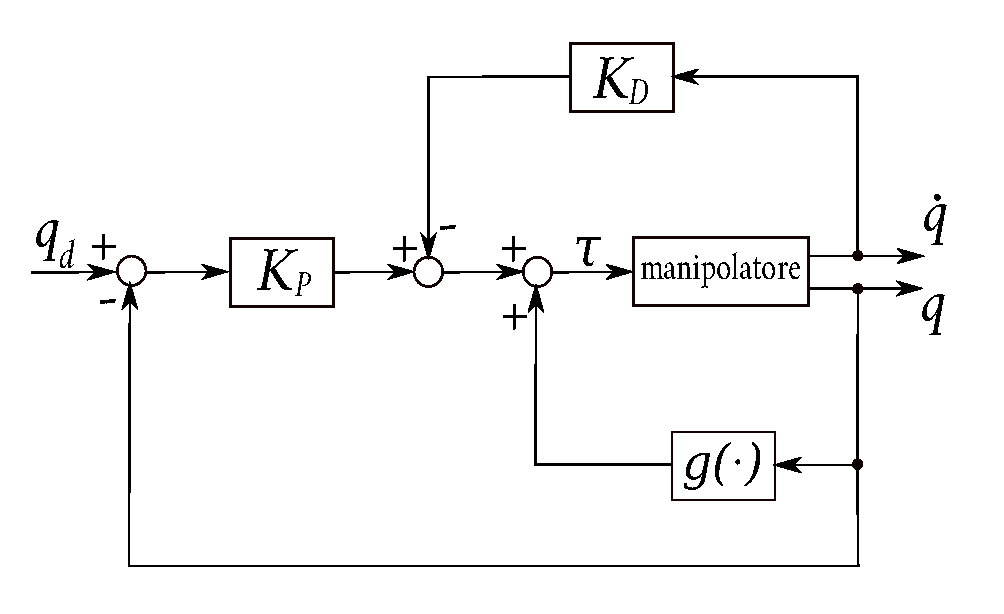
\includegraphics[scale=0.4]{centralizzatoPDgravita.pdf}
	\caption{Schema di controllo PD ai giunti con compensazione di gravità.}
\end{center}

\subsubsection{Discorso qualitativo:}
Quanto visto fino adesso \underline{dimostra} che qualunque postura di equilibrio del manipolatore risulta globalmente asintoticamente stabile se il controllo esplica un'azione lineare di tipo PD e un'azione non lineare di compensazione degli effetti gravitazionali. Pertanto la stabilità è assicurata con una scelta qualsiasi delle matrici $K_D$ e $K_P$ purchè siano definite positive.

\subsection{Controllo a Dinamica Inversa}
Consideriamo il problema dell'inseguimento di una traiettoria specificata nello spazio dei giunti. Il modello dinamico di un manipolatore a $n$ giunti è espresso dalla seguente relazione
\begin{equation}
	B(\underline{q})\underline{\ddot{q}} + n(\underline{q}, \underline{\dot{q}}) = \underline{\tau}
\end{equation}
con $n(\underline{q}, \underline{\dot{q}}) = C(\underline{q}, \underline{\dot{q}})\underline{\dot{q}} + F_v \underline{\dot{q}} + \underline{g}(\underline{q})$.

\paragraph{}
L'idea è quella di individuare un vettore di controllo $\underline{\tau}$, funzione dello stato del sistema, che sia in grado di realizzare relazioni ingresso-uscita che presentino caratteristiche lineari. L'obiettivo è quello di effettuare una \emph{linearizzazione esatta} mediante una retroazione \emph{non lineare} dello stato del sistema. Quindi \underline{non} una linearizzazione locale. 

Assumiamo la seguente legge di controllo,
\begin{equation}
	\underline{\tau} = \hat{B}(\underline{q})\underline{y} + \hat{n}(\underline{q}, \underline{\dot{q}})
\end{equation}
denominata \textbf{controllo a dinamica inversa} perchè si basa sul calcolo della dinamica inversa del manipolatore. A questo punto, poniamo l'uguaglianza
\begin{equation}
	B(\underline{q})\underline{\ddot{q}} + n(\underline{q}, \underline{\dot{q}}) = \hat{B}(\underline{q})\underline{y} + \hat{n}(\underline{q}, \underline{\dot{q}})
\end{equation}
e se la linearizzazione è esatta, otteniamo $\underline{n} = 0$, $B^{-1}\hat{B} = I$, ovvero un sistema costituito da un banco di integratori doppi.

Pertanto, il sistema è descritto dall'equazione $\underline{\ddot{q}} = \underline{y}$ con $\underline{y}$ nuovo vettore di ingresso la cui struttura deve ancora essere determinata.

\paragraph{}
Il sistema sotto la legge di controllo appena descritta, risulta \emph{lineare} e \emph{disaccoppiato} nei riguardi del nuovo ingresso $\underline{y}$. Ovvero, la componente $y_i$ influenza con un legame di doppia integrazione, solo la variabile di giunto $q_i$, indipendentemente dal moto degli altri giunti. Scegliamo,
\begin{equation}
	\underline{y} = \underline{\ddot{q}}_{\,d} + K_D \underline{\dot{e}} + K_P \underline{e}
\end{equation}
con $K_D$ e $K_P$ \emph{definite positive} e \emph{diagonali}, otteniamo il seguente sistema di equazioni
\begin{equation}
	\begin{cases}
		\underline{\ddot{q}} = \underline{y} \\
		\underline{y} = \underline{\ddot{q}}_{\,d} + K_D \underline{\dot{e}} + K_P \underline{e}
	\end{cases}
	\Rightarrow \quad
	\underbrace{\underline{\ddot{q}}_{\,d} - \underline{\ddot{q}}}_{\underline{\ddot{e}}} + K_D \underline{\dot{e}} + K_P \underline{e} = \underline{0}
\end{equation}
Quindi, il sistema risulta descritto dall'equazione,
\begin{equation}
	\underline{\ddot{e}} = -K_P \underline{e} - K_D \underline{\dot{e}} = 
	\begin{bmatrix}
		- K_P & - K_D
	\end{bmatrix}
	\underbrace{
	\begin{bmatrix}
		\underline{e} \\
		\underline{\dot{e}}
	\end{bmatrix}
	}_{\underline{\xi}}
\end{equation}
definendo $\underline{\xi}$ lo \emph{stato del sistema}, il sistema che si ottiene è $LTI$, scriviamo l'evoluzione dello stato,
\begin{equation}
	\underline{\dot{\xi}} = \frac{d}{dt} 
	\begin{bmatrix}
		\underline{e} \\
		\underline{\dot{e}}
	\end{bmatrix}
	= 
	\underbrace{
	\begin{bmatrix}
		0 & I \\
		-K_P & - K_D \\
	\end{bmatrix}
	}_{A}
	\begin{bmatrix}
		\underline{e} \\
		\underline{\dot{e}}
	\end{bmatrix}	
\end{equation} 
tutti gli autovalori di $A$ hanno parte reale negativa, quindi abbiamo la stabilità asintotica globale.

\paragraph{}
Troviamo gli autovalori con il polinomio caratteristico per un singolo asse $i$,
\begin{equation}
	\ddot{e}_i + K_{D_i} \dot{e}_i +K_{P_i} e_i = 0 \qquad \forall i = 1, \cdots, n
\end{equation}
con 
\begin{equation}
	\xi_i = 
	\begin{bmatrix}
		e_i \\
		\dot{e}_i \\
	\end{bmatrix}
	\quad
	A = 
	\begin{bmatrix}
		0 & 1 \\
		-K_{P_i} & -K_{D_i}
	\end{bmatrix}
\end{equation}
pertanto,
\begin{equation}
	\det(sI-A) = s^2 + K_{D_i}s + K_{P_i} = 0 \Rightarrow 
	\begin{cases}
		\zeta = \frac{K_{D_i}}{2 \sqrt{K_{P_i}}} \\
		\omega_n^2 = K_{P_i}
	\end{cases}
\end{equation}
con queste caratteristiche si garantisce inseguimento perfetto, e inoltre notiamo come l'errore converga a zero con una velocità di risposta dipendente dalle matrici $K_D$ e $K_P$. 

\subsubsection{Discorso qualitativo}
Lo schema del controllo a dinamica inversa risulta,
\begin{center}
	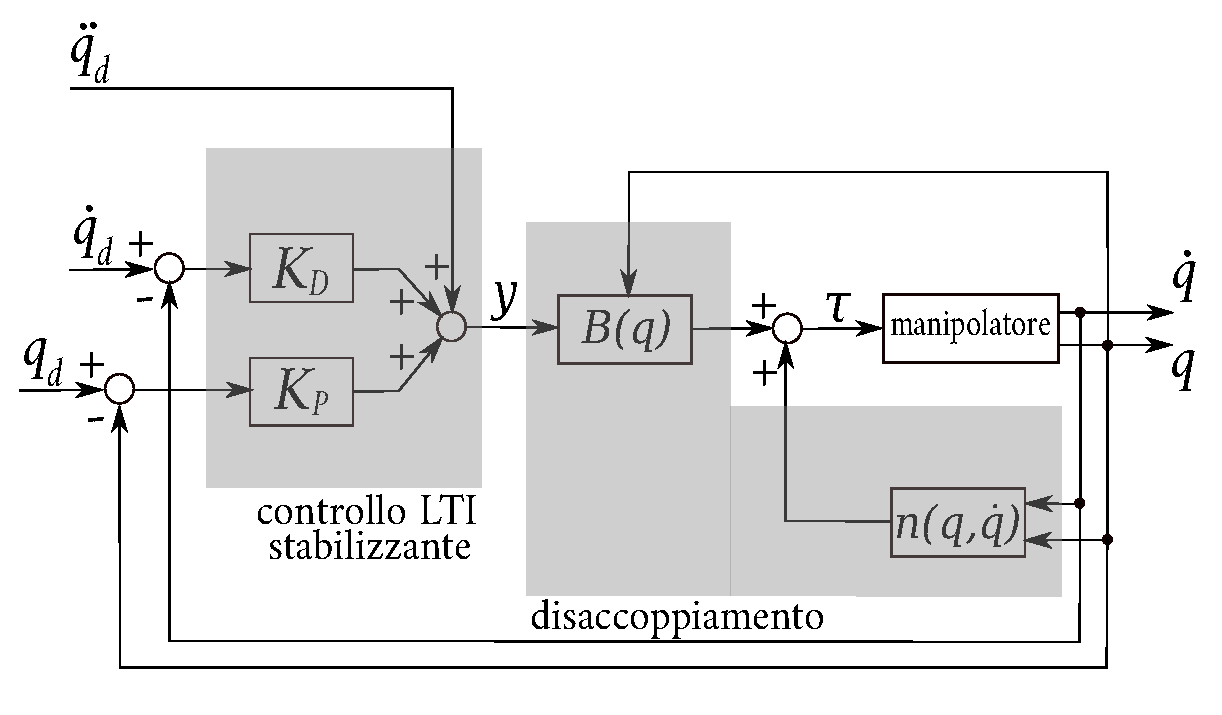
\includegraphics[scale=0.4]{centralizzatoDinamicaInversa.pdf}
	\caption{Schema di controllo a dinamica inversa ai giunti.}
\end{center}
dove possiamo notare la presenza di due anelli di retroazione,
\begin{itemize}
	\item l'anello interno basato sul modello dinamico del manipolatore e ha la funzione di rendere disponibile un legame ingresso-uscita lineare e disaccoppiato,
	\item l'anello esterno opera sull'errore e ha il compito di stabilizzare il sistema complessivo.
\end{itemize}
Questa tecnica di compensazione non lineare a disaccoppiamento è interessante perchè va ad effettuare una sostituzione della dinamica del manipolatore non lineare con $n$ sottosistemi lineari tra di loro non interagenti. 

\subsection{Computer Torque Control}
Questa tecnica è usata dalle più importanti aziende produttrici di Robot, si tratta di una compensazione in avanti a coppia precalcolata che fa uso sia del controllo centralizzato che di quello decentralizzato. 

Con riferimento allo schema più generale in Figura 9.20, la grandezza di uscita del PIDD$^2$ è costituita dalla funzione 
\begin{equation}
	a_2 \ddot{e} + a_1 \dot{e} a_0 e + a_{-1} \int_0^t e(\sigma) d\sigma
\end{equation}
che rappresenta l'evoluzione nel tempo dell'errore. Con riferimento allo schema seguente,
\begin{center}
	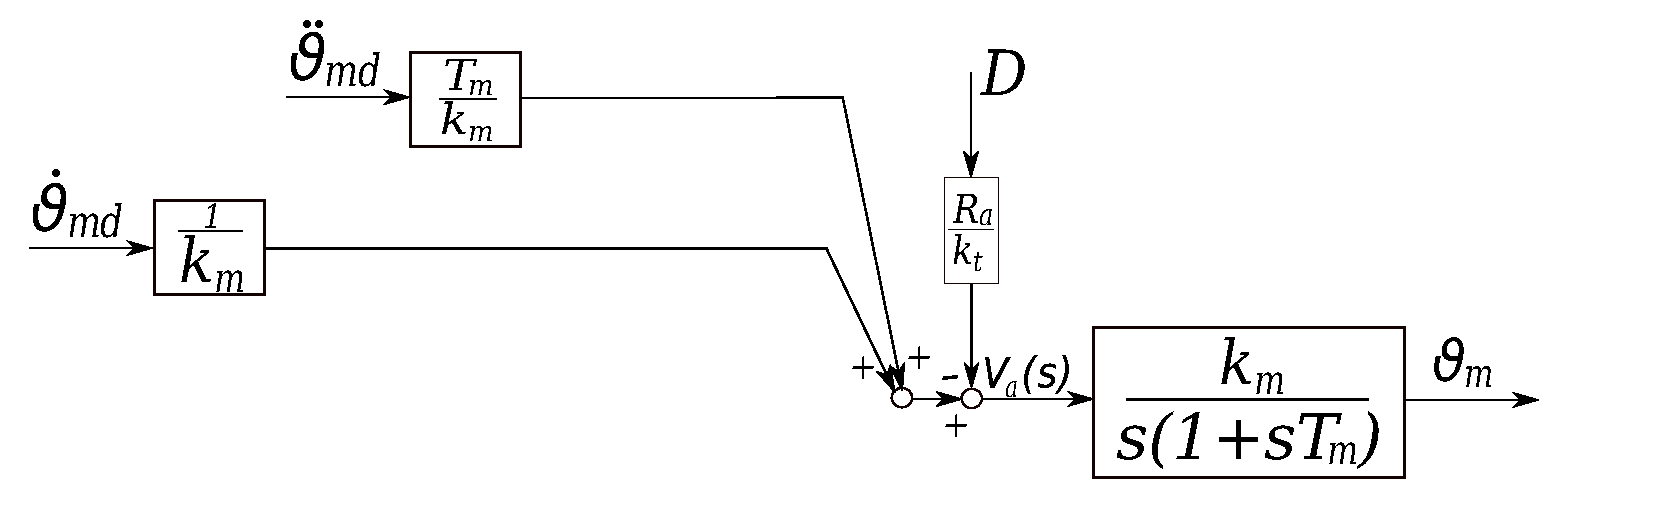
\includegraphics[scale=0.4]{dinamicaCTC.pdf}
\end{center}
costruiamo uno schema con
\begin{itemize}
	\item L'azione di \emph{feedback} rappresentata dalla ($9.50$)
	\item L'azione di \emph{feedforward} decentralizzata rappresentata da
		\begin{equation}
			\frac{T_m}{k_m} \ddot{\vartheta_{md}} + \frac{1}{k_m} \dot{\vartheta_{md}}
		\end{equation}
	\item Il disturbo, espresso come
		\begin{equation}
			-\frac{R_a}{k_t}\cdot d
		\end{equation}
\end{itemize}

\paragraph{}
L'obiettivo è quello di eliminare l'errore e il disturbo, ottenendo $\dot{\vartheta}_{md} = \dot{\vartheta_m}$ e $\ddot{\vartheta}_{md} = \ddot{\vartheta}_d$, pertanto desideriamo la seguente uguaglianza,
\begin{equation}
	a_2 \ddot{e} + a_1 \dot{e} a_0 e + a_{-1} \int_0^t e(\sigma) d\sigma + \frac{T_m}{k_m} \ddot{\vartheta_{md}} + \frac{1}{k_m} \dot{\vartheta_{md}} -\frac{R_a}{k_t}\cdot d = \frac{T_m}{k_m} \ddot{\vartheta_{m}} + \frac{1}{k_m} \dot{\vartheta_{m}}
\end{equation}
modificando i coefficienti ($a'_1 \triangleq a_1 + \frac{T_m}{k_m}$), scriviamo
\begin{equation}
	a'_2 \ddot{e} + a'_1 \dot{e} a'_0 e + a'_{-1} \int_0^t e(\sigma) d\sigma = \frac{R_a}{k_t} \cdot d
\end{equation}
tale equazione mostra che ogni traiettoria fisicamente eseguibile è asintoticamente seguita (a regime) se il termine di disturbo $d(t) = 0$.

\paragraph{}
La presenza del termine $d(t)$ comporta la nascita di un errore di inseguimento caratterizzato dalla \emph{f.d.t.}
\begin{equation}
	\frac{E(s)}{D(s)} = \frac{s \frac{R_a}{k_t}}{a'_2 s^3 + a'_1 s^2 + a'_0 s + a'_{-1}}
\end{equation}
notiamo che lo zero nell'origine va a reiettare a regime $D(s)$.

\paragraph{}
Si può aggiungere ai precedenti segnali di azioni in avanti un termine che sia in grado di compensare non gli effetti del disturbo ma il disturbo stesso. Siano $\underline{q}_{\,d}(t)$ la traiettoria desiderata per i giunti e $\underline{q}_{\,md}(t)$ la corrispondente traiettoria per gli attuatori. Utilizziamo l'azione in avanti
\begin{equation}
	R_a K_t^{-1} \underline{d}_{\,d}
\end{equation}
con
\begin{equation}
	\underline{d}_{\,d} = K_r^{-1} \Delta B(\underline{q}_{\,d}) K_r^{-1} \underline{\ddot{q}}_{\,md} + K_r^{-1} C(\underline{q}_{\,d}, \underline{\dot{q}}_{\,d}) K_r^{-1} \underline{\dot{q}}_{\,md} + K_r^{-1}\underline{g}(\underline{q}_{\,d})
\end{equation}
dove $R_a$ e $K_t$ denotano le matrici diagonali delle resistenze di armatura e delle costanti di coppia degli attuatori. L'azione in avanti della ($9.56$) tende a compensare il disturbo $\underline{d}$ espresso dalla ($9.5$). Le schema di questo controllo è
\begin{center}
	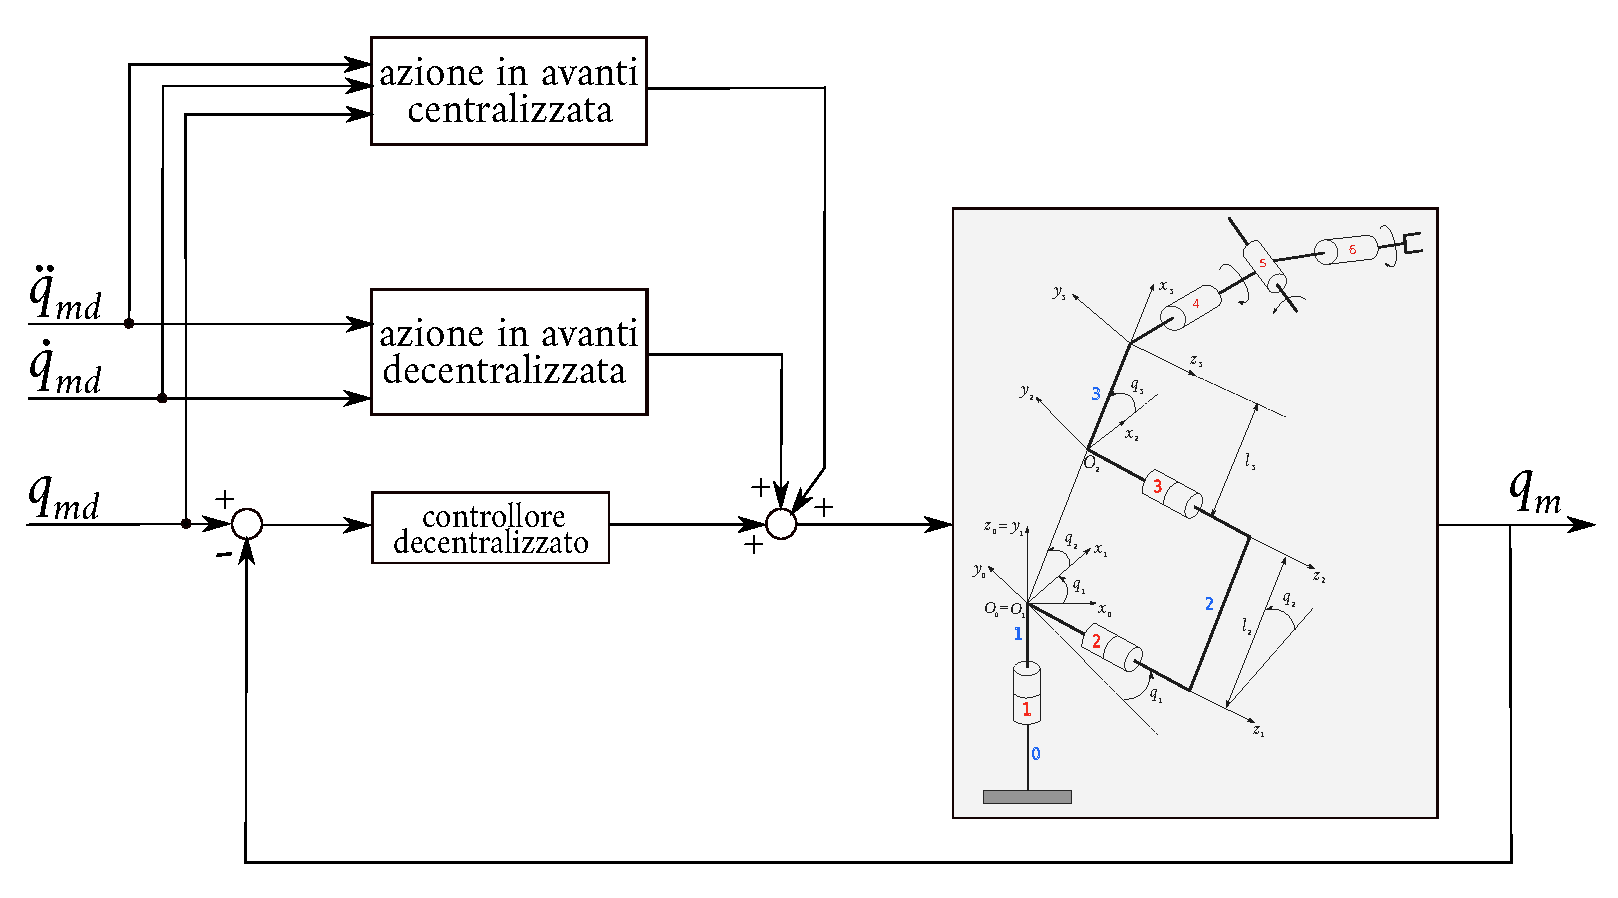
\includegraphics[scale=0.4]{ComputerTorqueControl.pdf}
	\caption{Schema di controllo CTC.}
\end{center}
e rappresenta in forma compatta il sistema di controllo di un manipolatore che realizza algoritmi di controllo del tipo  a coppia precalcolata. Notiamo

\begin{itemize}
	\item Il sistema di controllo in retroazione è rappresentativo degli $n$ sistemi di controllo dei singoli giunti considerati indipendenti, esso è \textbf{decentralizzato} in quanto il controllore $i$ di giunto elabora riferimenti e misure relativi a grandezze caratteristiche del solo giunto $i$.
	\item Le interazioni esistenti tra i diversi giunti, espresse dal disturbo $\underline{d}$, vengono compensate da \textbf{un'azione centralizzata} la cui funzione è quella di generare un'azione in avanti che dipende dai riferimenti di tutti i giunti e dal modello dinamico del manipolatore.
	\item L'azione centralizzata compensa i termini non lineari di accoppiamento dovuti alle coppie inerziali, di Coriolis, centrifughe e gravitazionali che dipendono dalla struttura e si modificano durante il movimento del manipolatore.
\end{itemize}